%%%%%%%%%%%%%%%%%%%%%%%%%%%%%%%%%%%%%%%%%
%
% Important note:
% Chapter heading images should have a 2:1 width:height ratio,
% e.g. 920px width and 460px height.
%
% The original template (the Legrand Orange Book Template) can be found here --> http://www.latextemplates.com/template/the-legrand-orange-book
%
% Original author of the Legrand Orange Book Template:
% Mathias Legrand (legrand.mathias@gmail.com) with modifications by: Vel (vel@latextemplates.com)
%
% Original License:
% CC BY-NC-SA 3.0 (http://creativecommons.org/licenses/by-nc-sa/3.0/)
%%%%%%%%%%%%%%%%%%%%%%%%%%%%%%%%%%%%%%%%%


%----------------------------------------------------------------------------------------
%	CETNTRAL VARIABLES
%----------------------------------------------------------------------------------------
\def\meinTitel{Sicherheit von KI-Systemen in Luftfahrtradarsystemen}
\def\TODO{\textcolor{Red}{TODO}}

\newcommand{\scriptTitle}{\meinTitel}
\newcommand{\scriptAuthor}{Tomy Hebel 78280}
\newcommand{\scriptSubject}{\meinTitel}
\newcommand{\scriptKeywords}{25sose\_Bachelor\_Thesis}
\newcommand{\scriptFaculty}{Maschinenbau und Mechatronik}
\newcommand{\scriptCourse}{Bachelor Thesis Sommersemester 2025}
\newcommand{\scriptPublisher}{Tomy Hebel}
\newcommand{\scriptWebsite}{https://ilias.h-ka.de}
\newcommand{\scriptLicense}{CC BY-NC-SA 3.0 (http://creativecommons.org/licenses/by-nc-sa/3.0/)}
\newcommand{\scriptEdition}{Erste Ausgabe, Stand: April 2025}

%----------------------------------------------------------------------------------------
%	PACKAGES AND OTHER DOCUMENT CONFIGURATIONS
%----------------------------------------------------------------------------------------

\documentclass[11pt,fleqn, oneside]{book} % Default font size and left-justified equations

%%%%%%%%%%%%%%%%%%%%%%%%%%%%%%%%%%%%%%%%%
% The Legrand Orange Book
% Structural Definitions File
% Version 2.1 (26/09/2018)
%
% Original author:
% Mathias Legrand (legrand.mathias@gmail.com) with modifications by:
% Vel (vel@latextemplates.com)
% 
% This file was downloaded from:
% http://www.LaTeXTemplates.com
%
% License:
% CC BY-NC-SA 3.0 (http://creativecommons.org/licenses/by-nc-sa/3.0/)
%
%%%%%%%%%%%%%%%%%%%%%%%%%%%%%%%%%%%%%%%%%

%	Abkürzungen
\usepackage{acronym}

%----------------------------------------------------------------------------------------
%	MARGINS
%----------------------------------------------------------------------------------------

\usepackage{geometry} % Required for adjusting page dimensions and margins

\geometry{
	paper=a4paper, % Paper size, change to letterpaper for US letter size
	top=3cm, % Top margin
	bottom=3cm, % Bottom margin
	left=3cm, % Left margin
	right=3cm, % Right margin
	headheight=14pt, % Header height
	footskip=1.4cm, % Space from the bottom margin to the baseline of the footer
	headsep=10pt, % Space from the top margin to the baseline of the header
	%showframe, % Uncomment to show how the type block is set on the page
}

\setlength{\parindent}{0pt} % Kein Einzug für die erste Zeile jedes Absatzes

%----------------------------------------------------------------------------------------
%	FONTS
%----------------------------------------------------------------------------------------
\usepackage[T1]{fontenc} % Ensures proper hyphenation of special characters
\usepackage[utf8]{inputenc} % Allows use of accented characters
\usepackage[ngerman]{babel} % German language support
\usepackage{csquotes} % Correct quotation marks in the respective language

\usepackage{avant} % Use the Avantgarde font for headings
\newcommand*{\avantstyle}{\fontfamily{pag}\selectfont}
\DeclareTextFontCommand{\avantfont}{\avantstyle}

\usepackage{plex-sans}

\renewcommand*\familydefault{\sfdefault} %% Only if the base font of the document is to be sans serif
%\usepackage{mathptmx} % Use the Adobe Times Roman as the default text font together with math symbols from the Sym­bol, Chancery and Com­puter Modern fonts

\usepackage{microtype} % Slightly tweak font spacing for aesthetics

%----------------------------------------------------------------------------------------
%	BIBLIOGRAPHY AND INDEX
%----------------------------------------------------------------------------------------

\usepackage[style=numeric,citestyle=numeric,sorting=nyt,sortcites=true,autopunct=true,hyperref=true,abbreviate=false,backref=true,backend=biber]{biblatex}
\addbibresource{bibliography.bib} % BibTeX bibliography file
\defbibheading{bibempty}{}

\usepackage{calc} % For simpler calculation - used for spacing the index letter headings correctly
\usepackage{makeidx} % Required to make an index
\makeindex % Tells LaTeX to create the files required for indexing

%----------------------------------------------------------------------------------------
%	DIGITAL LOGIC & ELECTRONICS
%----------------------------------------------------------------------------------------

\usepackage[european, RPvoltages]{circuitikz}

%----------------------------------------------------------------------------------------
%	MAIN TABLE OF CONTENTS
%----------------------------------------------------------------------------------------

\usepackage{titletoc} % Required for manipulating the table of contents

\contentsmargin{0cm} % Removes the default margin

% Part text styling (this is mostly taken care of in the PART HEADINGS section of this file)
\titlecontents{part}
	[0cm] % Left indentation
	{\addvspace{20pt}\bfseries} % Spacing and font options for parts
	{}
	{}
	{}

% Chapter text styling
\titlecontents{chapter}
	[1.25cm] % Left indentation
	{\addvspace{12pt}\large\sffamily\bfseries} % Spacing and font options for chapters
	{\color{ThemeColor}\contentslabel[\Large\thecontentslabel]{1.25cm}\color{ThemeColor}} % Formatting of numbered sections of this type
	{\color{ThemeColor}} % Formatting of numberless sections of this type
	{\color{ThemeColor}\normalsize\;\titlerule*[.5pc]{.}\;\thecontentspage} % Formatting of the filler to the right of the heading and the page number

% Section text styling
\titlecontents{section}
	[1.25cm] % Left indentation
	{\addvspace{3pt}\sffamily\bfseries} % Spacing and font options for sections
	{\contentslabel[\thecontentslabel]{1.25cm}} % Formatting of numbered sections of this type
	{} % Formatting of numberless sections of this type
	{\hfill\color{black}\thecontentspage} % Formatting of the filler to the right of the heading and the page number

% Subsection text styling
\titlecontents{subsection}
	[1.25cm] % Left indentation
	{\addvspace{1pt}\sffamily\small} % Spacing and font options for subsections
	{\contentslabel[\thecontentslabel]{1.25cm}} % Formatting of numbered sections of this type
	{} % Formatting of numberless sections of this type
	{\ \titlerule*[.5pc]{.}\;\thecontentspage} % Formatting of the filler to the right of the heading and the page number

% Figure text styling
\titlecontents{figure}
	[1.25cm] % Left indentation
	{\addvspace{1pt}\sffamily\small} % Spacing and font options for figures
	{\thecontentslabel\hspace*{1em}} % Formatting of numbered sections of this type
	{} % Formatting of numberless sections of this type
	{\ \titlerule*[.5pc]{.}\;\thecontentspage} % Formatting of the filler to the right of the heading and the page number

% Table text styling
\titlecontents{table}
	[1.25cm] % Left indentation
	{\addvspace{1pt}\sffamily\small} % Spacing and font options for tables
	{\thecontentslabel\hspace*{1em}} % Formatting of numbered sections of this type
	{} % Formatting of numberless sections of this type
	{\ \titlerule*[.5pc]{.}\;\thecontentspage} % Formatting of the filler to the right of the heading and the page number

%----------------------------------------------------------------------------------------
%	MINI TABLE OF CONTENTS IN PART HEADS
%----------------------------------------------------------------------------------------

% To override the existing colorred text
\newcommand{\absolutetextcolor}[2]{%
    \textcolor{#1}{%
        \renewcommand\textcolor[2][]{}%
    #2}%
}

% Chapter text styling
\titlecontents{lchapter}
	[0em] % Left indentation
	{\addvspace{15pt}\large\sffamily\bfseries} % Spacing and font options for chapters
	{\color{white}\contentslabel[\Large\thecontentslabel]{1.25cm}\color{white}} % Chapter number
	{\absolutetextcolor{white}}
	{\color{white}\normalsize\sffamily\bfseries\;\titlerule*[.5pc]{.}\;\thecontentspage} % Page number

% Section text styling
\titlecontents{lsection}
	[0em] % Left indentation
	{\color{white}\sffamily\small} % Spacing and font options for sections
	{\contentslabel[\thecontentslabel]{1.25cm}} % Section number
	{}
	{}

% Subsection text styling (note these aren't shown by default, display them by searchings this file for tocdepth and reading the commented text)
\titlecontents{lsubsection}
	[.5em] % Left indentation
	{\color{white}\sffamily\footnotesize} % Spacing and font options for subsections
	{\contentslabel[\thecontentslabel]{1.25cm}}
	{}
	{}

%----------------------------------------------------------------------------------------
%	HEADERS AND FOOTERS
%----------------------------------------------------------------------------------------

\usepackage{fancyhdr} % Required for header and footer configuration

\pagestyle{fancy} % Enable the custom headers and footers

\renewcommand{\chaptermark}[1]{\markboth{\sffamily\normalsize\bfseries\chaptername\ \thechapter.\ #1}{}} % Styling for the current chapter in the header
\renewcommand{\sectionmark}[1]{\markright{\sffamily\normalsize\thesection\hspace{5pt}#1}{}} % Styling for the current section in the header

\fancyhf{} % Clear default headers and footers
\fancyhead[LE,RO]{\sffamily\normalsize\thepage} % Styling for the page number in the header
\fancyhead[LO]{\rightmark} % Print the nearest section name on the left side of odd pages
\fancyhead[RE]{\leftmark} % Print the current chapter name on the right side of even pages
%\fancyfoot[C]{\thepage} % Uncomment to include a footer

\renewcommand{\headrulewidth}{0.5pt} % Thickness of the rule under the header

\fancypagestyle{plain}{% Style for when a plain pagestyle is specified
	\fancyhead{}\renewcommand{\headrulewidth}{0pt}%
}

% Removes the header from odd empty pages at the end of chapters
\makeatletter	% Einkommentieren für leeere Seiten /page /newpage /ungerade seiten zahlen
%\renewcommand{\cleardoublepage}{
%\clearpage\ifodd\c@page\else
%\hbox{}
%\vspace*{\fill}
%\thispagestyle{empty}
%\newpage
%\fi}

%----------------------------------------------------------------------------------------
%	THEOREM STYLES
%----------------------------------------------------------------------------------------

\usepackage{amsmath,amsfonts,amssymb,amsthm} % For math equations, theorems, symbols, etc

\newcommand{\intoo}[2]{\mathopen{]}#1\,;#2\mathclose{[}}
\newcommand{\ud}{\mathop{\mathrm{{}d}}\mathopen{}}
\newcommand{\intff}[2]{\mathopen{[}#1\,;#2\mathclose{]}}
\renewcommand{\qedsymbol}{$\blacksquare$}
\newtheorem{notation}{Notation}[chapter]

% Boxed/framed environments
\newtheoremstyle{ThemeColornumbox}% Theorem style name
{0pt}% Space above
{0pt}% Space below
{\normalfont}% Body font
{}% Indent amount
{\small\bf\sffamily\color{ThemeColor}}% Theorem head font
{\;}% Punctuation after theorem head
{0.25em}% Space after theorem head
{\small\sffamily\color{ThemeColor}\thmname{#1}\nobreakspace\thmnumber{\@ifnotempty{#1}{}\@upn{#2}}% Theorem text (e.g. Theorem 2.1)
\thmnote{\nobreakspace\the\thm@notefont\sffamily\bfseries\color{black}---\nobreakspace#3.}} % Optional theorem note

\newtheoremstyle{blacknumex}% Theorem style name
{5pt}% Space above
{5pt}% Space below
{\normalfont}% Body font
{} % Indent amount
{\small\bf\sffamily}% Theorem head font
{\;}% Punctuation after theorem head
{0.25em}% Space after theorem head
{\small\sffamily{\tiny\ensuremath{\blacksquare}}\nobreakspace\thmname{#1}\nobreakspace\thmnumber{\@ifnotempty{#1}{}\@upn{#2}}% Theorem text (e.g. Theorem 2.1)
\thmnote{\nobreakspace\the\thm@notefont\sffamily\bfseries---\nobreakspace#3.}}% Optional theorem note

\newtheoremstyle{blacknumbox} % Theorem style name
{0pt}% Space above
{0pt}% Space below
{\normalfont}% Body font
{}% Indent amount
{\small\bf\sffamily}% Theorem head font
{\;}% Punctuation after theorem head
{0.25em}% Space after theorem head
{\small\sffamily\thmname{#1}\nobreakspace\thmnumber{\@ifnotempty{#1}{}\@upn{#2}}% Theorem text (e.g. Theorem 2.1)
\thmnote{\nobreakspace\the\thm@notefont\sffamily\bfseries---\nobreakspace#3.}}% Optional theorem note

% Non-boxed/non-framed environments
\newtheoremstyle{ThemeColornum}% Theorem style name
{5pt}% Space above
{5pt}% Space below
{\normalfont}% Body font
{}% Indent amount
{\small\bf\sffamily\color{ThemeColor}}% Theorem head font
{\;}% Punctuation after theorem head
{0.25em}% Space after theorem head
{\small\sffamily\color{ThemeColor}\thmname{#1}\nobreakspace\thmnumber{\@ifnotempty{#1}{}\@upn{#2}}% Theorem text (e.g. Theorem 2.1)
\thmnote{\nobreakspace\the\thm@notefont\sffamily\bfseries\color{black}---\nobreakspace#3.}} % Optional theorem note
\makeatother

% Defines the theorem text style for each type of theorem to one of the three styles above
%\newcounter{dummy} 
%\numberwithin{dummy}{section}
%\theoremstyle{ThemeColornumbox}
%\newtheorem{theoremeT}[dummy]{Theorem}
%\newtheorem{problem}{Problem}[chapter]
%\newtheorem{exerciseT}{Exercise}[chapter]
%\theoremstyle{blacknumex}
%\newtheorem{exampleT}{Example}[chapter]
%\theoremstyle{blacknumbox}
%\newtheorem{vocabulary}{Vocabulary}[chapter]
%\newtheorem{definitionT}{Definition}[section]
%\newtheorem{corollaryT}[dummy]{Corollary}
%\theoremstyle{ThemeColornum}
%\newtheorem{proposition}[dummy]{Proposition}

% Deutsche Begriffe fuer Theorem-Boxen
\newcounter{dummy} 
\numberwithin{dummy}{section}
\theoremstyle{ThemeColornumbox}
\newtheorem{theoremeT}[dummy]{Satz}
\newtheorem{problem}{Problem}[chapter]
\newtheorem{exerciseT}{\"Ubung}[chapter]
\theoremstyle{blacknumex}
\newtheorem{exampleT}{Beispiel}[chapter]
\theoremstyle{blacknumbox}
\newtheorem{vocabulary}{W\"orterverzeichnis }[chapter]
\newtheorem{definitionT}{Definition}[section]
\newtheorem{corollaryT}[dummy]{Folgerung}
\theoremstyle{ThemeColornum}
\newtheorem{proposition}[dummy]{These}


%----------------------------------------------------------------------------------------
%	DEFINITION OF COLORED BOXES
%----------------------------------------------------------------------------------------

\RequirePackage[framemethod=default]{mdframed} % Required for creating the theorem, definition, exercise and corollary boxes

% Theorem box
\newmdenv[skipabove=7pt,
skipbelow=7pt,
backgroundcolor=black!5,
linecolor=ThemeColor,
innerleftmargin=5pt,
innerrightmargin=5pt,
innertopmargin=5pt,
leftmargin=0cm,
rightmargin=0cm,
innerbottommargin=5pt]{tBox}

% Exercise box	  
\newmdenv[skipabove=7pt,
skipbelow=7pt,
rightline=false,
leftline=true,
topline=false,
bottomline=false,
backgroundcolor=ThemeColor!10,
linecolor=ThemeColor,
innerleftmargin=5pt,
innerrightmargin=5pt,
innertopmargin=5pt,
innerbottommargin=5pt,
leftmargin=0cm,
rightmargin=0cm,
linewidth=4pt]{eBox}	

% Definition box
\newmdenv[skipabove=7pt,
skipbelow=7pt,
rightline=false,
leftline=true,
topline=false,
bottomline=false,
linecolor=ThemeColor,
innerleftmargin=5pt,
innerrightmargin=5pt,
innertopmargin=0pt,
leftmargin=0cm,
rightmargin=0cm,
linewidth=4pt,
innerbottommargin=0pt]{dBox}	

% Corollary box
\newmdenv[skipabove=7pt,
skipbelow=7pt,
rightline=false,
leftline=true,
topline=false,
bottomline=false,
linecolor=gray,
backgroundcolor=black!5,
innerleftmargin=5pt,
innerrightmargin=5pt,
innertopmargin=5pt,
leftmargin=0cm,
rightmargin=0cm,
linewidth=4pt,
innerbottommargin=5pt]{cBox}

% Creates an environment for each type of theorem and assigns it a theorem text style from the "Theorem Styles" section above and a colored box from above
\newenvironment{theorem}{\begin{tBox}\begin{theoremeT}}{\end{theoremeT}\end{tBox}}
\newenvironment{exercise}{\begin{eBox}\begin{exerciseT}}{\hfill{\color{ThemeColor}\tiny\ensuremath{\blacksquare}}\end{exerciseT}\end{eBox}}				  
\newenvironment{definition}{\begin{dBox}\begin{definitionT}}{\end{definitionT}\end{dBox}}	
\newenvironment{example}{\begin{exampleT}}{\hfill{\tiny\ensuremath{\blacksquare}}\end{exampleT}}		
\newenvironment{corollary}{\begin{cBox}\begin{corollaryT}}{\end{corollaryT}\end{cBox}}	

%----------------------------------------------------------------------------------------
%	REMARK ENVIRONMENT
%----------------------------------------------------------------------------------------

\newenvironment{remark}{\par\vspace{10pt}\small % Vertical white space above the remark and smaller font size
\begin{list}{}{
\leftmargin=35pt % Indentation on the left
\rightmargin=25pt}\item\ignorespaces % Indentation on the right
\makebox[-2.5pt]{\begin{tikzpicture}[overlay]
\node[draw=ThemeColor,line width=1pt,circle,fill=ThemeColor!25,font=\sffamily\bfseries,inner sep=2pt,outer sep=0pt] at (-15pt,0pt){\textcolor{ThemeColor}{R}};\end{tikzpicture}} % Orange R in a circle
\advance\baselineskip -1pt}{\end{list}\vskip5pt} % Tighter line spacing and white space after remark

%----------------------------------------------------------------------------------------
%	SECTION NUMBERING IN THE MARGIN
%----------------------------------------------------------------------------------------

\makeatletter
\renewcommand{\@seccntformat}[1]{\llap{\textcolor{ThemeColor}{\csname the#1\endcsname}\hspace{1em}}}                    
\renewcommand{\section}{\@startsection{section}{1}{\z@}
{-4ex \@plus -1ex \@minus -.4ex}
{1ex \@plus.2ex }
{\normalfont\large\sffamily\bfseries}}
\renewcommand{\subsection}{\@startsection {subsection}{2}{\z@}
{-3ex \@plus -0.1ex \@minus -.4ex}
{0.5ex \@plus.2ex }
{\normalfont\sffamily\bfseries}}
\renewcommand{\subsubsection}{\@startsection {subsubsection}{3}{\z@}
{-2ex \@plus -0.1ex \@minus -.2ex}
{.2ex \@plus.2ex }
{\normalfont\small\sffamily\bfseries}}                        
\renewcommand\paragraph{\@startsection{paragraph}{4}{\z@}
{-2ex \@plus-.2ex \@minus .2ex}
{.1ex}
{\normalfont\small\sffamily\bfseries}}

%----------------------------------------------------------------------------------------
%	PART HEADINGS
%----------------------------------------------------------------------------------------

% Numbered part in the table of contents
\newcommand{\@mypartnumtocformat}[2]{%
	\setlength\fboxsep{0pt}%
	\noindent\colorbox{ThemeColor}{\strut\parbox[c][.7cm]{\ecart}{\color{white}\Large\sffamily\bfseries\centering#1}}\hskip\esp\colorbox{ThemeColor}{\strut\parbox[c][.7cm]{\linewidth-\ecart-\esp}{\color{white}\Large\sffamily\centering#2}}%
}

% Unnumbered part in the table of contents
\newcommand{\@myparttocformat}[1]{%
	\setlength\fboxsep{0pt}%
	\noindent\colorbox{ThemeColor}{\strut\parbox[c][.7cm]{\linewidth}{\Large\sffamily\centering#1}}%
}

\newlength\esp
\setlength\esp{4pt}
\newlength\ecart
\setlength\ecart{1.2cm-\esp}
\newcommand{\thepartimage}{}%
\newcommand{\partimage}[1]{\renewcommand{\thepartimage}{#1}}%
\def\@part[#1]#2{%
\ifnum \c@secnumdepth >-2\relax%
\refstepcounter{part}%
\addcontentsline{toc}{part}{\texorpdfstring{\protect\@mypartnumtocformat{\thepart}{#1}}{\partname~\thepart\ ---\ #1}}
\else%
\addcontentsline{toc}{part}{\texorpdfstring{\protect\@myparttocformat{#1}}{#1}}%
\fi%
\startcontents%
\markboth{}{}%
{\thispagestyle{empty}%
\begin{tikzpicture}[remember picture,overlay]%
\node at (current page.north west){\begin{tikzpicture}[remember picture,overlay]%	
\fill[ThemeColor](0cm,0cm) rectangle (\paperwidth,-\paperheight);
\node[anchor=north] at (5.5cm,-3.25cm){\color{white}\fontsize{220}{100}\sffamily\bfseries\thepart}; 
\node[anchor=south east] at (\paperwidth-1cm,-\paperheight+1cm){\parbox[t][][t]{8.5cm}{
\printcontents{l}{0}{\setcounter{tocdepth}{1}}% The depth to which the Part mini table of contents displays headings; 0 for chapters only, 1 for chapters and sections and 2 for chapters, sections and subsections
}};
\node[anchor=north east] at (\paperwidth-1.5cm,-3.25cm){\parbox[t][][t]{8cm}{\strut\raggedleft\color{white}\fontsize{30}{30}\sffamily\bfseries#2}};
\end{tikzpicture}};
\end{tikzpicture}}%
\@endpart}
\def\@spart#1{%
\startcontents%
\phantomsection
{\thispagestyle{empty}%
\begin{tikzpicture}[remember picture,overlay]%
\node at (current page.north west){\begin{tikzpicture}[remember picture,overlay]%	
\fill[ThemeColor!20](0cm,0cm) rectangle (\paperwidth,-\paperheight);
\node[anchor=north east] at (\paperwidth-1.5cm,-3.25cm){\parbox[t][][t]{15cm}{\strut\raggedleft\color{white}\fontsize{30}{30}\sffamily\bfseries#1}};
\end{tikzpicture}};
\end{tikzpicture}}
\addcontentsline{toc}{part}{\texorpdfstring{%
\setlength\fboxsep{0pt}%
\noindent\protect\colorbox{ThemeColor!40}{\strut\protect\parbox[c][.7cm]{\linewidth}{\Large\sffamily\protect\centering #1\quad\mbox{}}}}{#1}}%
\@endpart}
\def\@endpart{\vfil\newpage
\if@twoside
\if@openright
\null
\thispagestyle{empty}%
\newpage
\fi
\fi
\if@tempswa
\twocolumn
\fi}

%----------------------------------------------------------------------------------------
%	CHAPTER HEADINGS
%----------------------------------------------------------------------------------------

% A switch to conditionally include a picture, implemented by Christian Hupfer
\newif\ifusechapterimage
\usechapterimagetrue
\newcommand{\thechapterimage}{}%
\newcommand{\chapterimage}[1]{\ifusechapterimage\renewcommand{\thechapterimage}{#1}\fi}%
\newcommand{\autodot}{.}
\def\@makechapterhead#1{%
	{\parindent \z@ \raggedright \normalfont
		\ifnum \c@secnumdepth >\m@ne

		\if@mainmatter %checks, if chapter is part of mainmatter (no appendix/other)
        \begin{tikzpicture}[remember picture,overlay]
			\node at (current page.north west)
			{\begin{tikzpicture}[remember picture,overlay]
					\node[anchor=north west,inner sep=0pt] at (0,0) {\ifusechapterimage\includegraphics[width=\paperwidth]{\thechapterimage}\fi};

                    %conditionally set position of title
                    \ifusechapterimage
					\draw[anchor=west] (\Gm@lmargin-0cm,-9cm) node [minimum height=2cm, line width=0pt,rounded corners=0pt,draw=white,fill=white,fill opacity=1,inner sep=10pt] {\huge\bfseries\color{ThemeColor}\thechapter\autodot ~#1 \strut};
					\draw[anchor=east] (\Gm@lmargin-0cm,-9cm) node [minimum width=1cm, minimum height=2cm, line width=0pt,rounded corners=0pt, draw=ThemeColor,fill=ThemeColor,fill opacity=1] {};

                    \else
                    \draw[anchor=west] (\Gm@lmargin-0cm,-3cm) node [minimum height=2cm, line width=0pt,rounded corners=0pt,draw=white,fill=white,fill opacity=1,inner sep=10pt] {\huge\bfseries\color{ThemeColor}\thechapter\autodot ~#1 \strut};
					\draw[anchor=east] (\Gm@lmargin-0cm,-3cm) node [minimum width=1cm, minimum height=2cm, line width=0pt,rounded corners=0pt, draw=ThemeColor,fill=ThemeColor,fill opacity=1] {};
                    \fi

			\end{tikzpicture}};
		\end{tikzpicture}

		\else  %draw title for unnumbered chapters --> not @mainmatter
		\begin{tikzpicture}[remember picture,overlay]
			\node at (current page.north west)
			{\begin{tikzpicture}[remember picture,overlay]
					\node[anchor=north west,inner sep=0pt] at (0,0) {\ifusechapterimage\includegraphics[width=\paperwidth]{\thechapterimage}\fi};
     
					\ifusechapterimage
                    \draw[anchor=west] (\Gm@lmargin-0cm,-9cm) node [minimum height=2cm, line width=0pt,rounded corners=0pt,draw=white,fill=white,fill opacity=1,inner sep=10pt] {\huge\bfseries\color{ThemeColor} #1 \strut};
					\draw[anchor=east] (\Gm@lmargin-0cm,-9cm) node [minimum width=1cm, minimum height=2cm, line width=0pt,rounded corners=0pt,draw=ThemeColor,fill=ThemeColor,fill opacity=1] {};
     
                    \else
                    \draw[anchor=west] (\Gm@lmargin-0cm,-3cm) node [minimum height=2cm, line width=0pt,rounded corners=0pt,draw=white,fill=white,fill opacity=1,inner sep=10pt] {\huge\bfseries\color{ThemeColor} #1 \strut};
					\draw[anchor=east] (\Gm@lmargin-0cm,-3cm) node [minimum width=1cm, minimum height=2cm, line width=0pt,rounded corners=0pt,draw=ThemeColor,fill=ThemeColor,fill opacity=1] {};
                    \fi
     
			\end{tikzpicture}};
		\end{tikzpicture}
  
		\fi\fi\par

        \ifusechapterimage
        \vspace*{250\p@}
        \else
        \vspace*{50\p@}
        \fi   
    }}

\def\@makeschapterhead#1{ %make chapterheads for appendix 
	\begin{tikzpicture}[remember picture,overlay]
		\node at (current page.north west)
		{\begin{tikzpicture}[remember picture,overlay]
				\node[anchor=north west,inner sep=0pt] at (0,0) {\ifusechapterimage\includegraphics[width=\paperwidth]{\thechapterimage}\fi};

                \ifusechapterimage
				\draw[anchor=west] (\Gm@lmargin-0cm,-9cm) node [minimum height=2cm, line width=0pt,rounded corners=0pt,draw=white,fill=white,fill opacity=1,inner sep=10pt] {\huge\bfseries\color{ThemeColor} #1 \strut};
				\draw[anchor=east] (\Gm@lmargin-0cm,-9cm) node [minimum width=1cm, minimum height=2cm, line width=0pt,rounded corners=0pt,draw=ThemeColor,fill=ThemeColor,fill opacity=1] {};
                
                \else
                \draw[anchor=west] (\Gm@lmargin-0cm,-3cm) node [minimum height=2cm, line width=0pt,rounded corners=0pt,draw=white,fill=white,fill opacity=1,inner sep=10pt] {\huge\bfseries\color{ThemeColor} #1 \strut};
				\draw[anchor=east] (\Gm@lmargin-0cm,-3cm) node [minimum width=1cm, minimum height=2cm, line width=0pt,rounded corners=0pt,draw=ThemeColor,fill=ThemeColor,fill opacity=1] {};
                \fi
    
		\end{tikzpicture}};
	\end{tikzpicture}

    \ifusechapterimage
	\par\vspace*{250\p@}
    \else
    \par\vspace*{50\p@}
    \fi
 }
\makeatother

%----------------------------------------------------------------------------------------
%	LINKS
%----------------------------------------------------------------------------------------

\usepackage{hyperref}
\hypersetup{hidelinks, colorlinks=false,breaklinks=true,urlcolor=ThemeColor,bookmarksopen=false}

\usepackage{bookmark}
\bookmarksetup{
open,
numbered,
addtohook={%
\ifnum\bookmarkget{level}=0 % chapter
\bookmarksetup{bold}%
\fi
\ifnum\bookmarkget{level}=-1 % part
\bookmarksetup{color=ThemeColor,bold}%
\fi
}
}

%----------------------------------------------------------------------------------------
%	Ordnerstruktur und Dateien darstellen
%----------------------------------------------------------------------------------------

\usepackage[edges]{forest}

\definecolor{foldercolor}{RGB}{124,166,198}

\tikzset{pics/folder/.style={code={%
    \node[inner sep=0pt, minimum size=#1](-foldericon){};
    \node[folder style, inner sep=0pt, minimum width=0.3*#1, minimum height=0.6*#1, above right, xshift=0.05*#1] at (-foldericon.west){};
    \node[folder style, inner sep=0pt, minimum size=#1] at (-foldericon.center){};}
    },
    pics/folder/.default={20pt},
    folder style/.style={draw=foldercolor!80!black,top color=foldercolor!40,bottom color=foldercolor}
}

\forestset{is file/.style={edge path'/.expanded={%
        ([xshift=\forestregister{folder indent}]!u.parent anchor) |- (.child anchor)},
        inner sep=1pt,, inner ysep=-2pt},
    this folder size/.style={edge path'/.expanded={%
        ([xshift=\forestregister{folder indent}]!u.parent anchor) |- (.child anchor) pic[solid]{folder=#1}}, inner ysep=0.6*#1},
    folder tree indent/.style={before computing xy={l=#1}},
    folder icons/.style={folder, this folder size=#1, folder tree indent=3*#1},
    folder icons/.default={12pt},
} % Insert the structure.tex file which contains the majority of the structure behind the template

%----------------------------------------------------------------------------------------
%	VARIOUS REQUIRED PACKAGES AND CONFIGURATIONS
%----------------------------------------------------------------------------------------

\usepackage{graphicx} % Required for including pictures
\graphicspath{{Pictures/}} % Specifies the directory where pictures are stored

\usepackage{caption}
\usepackage{subcaption}

\usepackage{lipsum} % Inserts dummy text
\usepackage{tikz} % Required for drawing custom shapes

\usepackage{enumitem} % Customize lists
\setlist{nolistsep} % Reduce spacing between bullet points and numbered lists

\usepackage{booktabs} % Required for nicer horizontal rules in tables

\usepackage{xcolor} % Required for specifying colors by name

\usepackage[section]{placeins} % Graphics and tables are forced to be set before the beginning of a new section. Althoug this does not work with subsections. But you can use \FloatBarrier before a subsection to prevent this.

\usepackage[ngerman]{babel} % if you want to write in german
%\usepackage[english,ngerman]{babel} % for a multi-language file
\usepackage{csquotes} % korrekte Darstellung von Anführungszeichen

\usepackage{pdfpages}

\usepackage{listings}
%----------------------------------------------------------------------------------------
% User created custom commands
%----------------------------------------------------------------------------------------

\usepackage{float}
% 'OneFIGure' erzeugt eine Figure mit einem Bild darin. 
% Nutzung: \ofig{caption}{image_filename (ohne Dateiendung)}{image_width}
\newcommand{\ofig}[3]{
	\begin{figure}[h]
		\centering\includegraphics[width=#3]{#2}
		\caption{#1}
		\label{fig:#2}
	\end{figure}
}

% 'PlaceholderFIGure' erzeugt Figure mit dem Platzhalterbild darin. 
% Nutzung: \pfig{string caption}
\newcommand{\pfig}[1]{
	\ofig{#1}{placeholder}{\linewidth}
}

% 'Create TikZ Titlepage' creates the Title Page and changes the colour scheme corresponding to the faculty
% Nutzung: \createTikZTitlePage{Text: Faculty}{Text: Title}{Text: Authors}
\newcommand{\createTikZTitlePage}[3]{
	\begingroup
	\thispagestyle{empty} % Suppress headers and footers on the title page
	\begin{tikzpicture}[remember picture,overlay]

	%%% node coordinates A4 %%%
		% specify absolute placement on page, figures will be drawn relative to those
		\coordinate (UoAS) at ($ (current page.north west) + (2,-2) $);
		\coordinate (Faculty) at ($ (UoAS) + (0,-2) $);
		\coordinate (Title) at ($ (current page.north west) + (2,-11.5) $);
		\coordinate (Authors) at ($ (current page.south west) + (2,1.5) $);
		\coordinate (BackgroundPic) at ($ (current page.south) + (0,3) $);
		\coordinate (ColorBlock) at (0,-16);
		\coordinate (H) at ($ (current page.north east) + (8,-0.8) $);
		\coordinate (K) at ($ (H) + (0,-18) $);
		\coordinate (A) at ($ (K) + (0,-8.6) $);
		
	%%% Background Picture %%%
		\node[above, inner sep=0pt] (Hinterlegbild) at (BackgroundPic)
		% upper picture boundary needs to be at 3/5 of Page, which is 17.82cm. It starts 3cm from bottom so: 14.82cm
		% {\includegraphics[height=14.82cm]{../Pictures/csm_HKA_Image_2017_EIT_9006_92a30c9926.jpg}}; 
		{
\includegraphics[height=14.82cm]{../Bilder_und_Co/ai_safety_front_page.png}}; 
		
	%%% Colored, 3cm high, Box under Picture %%%
		\path[fill=ThemeColor] (current page.south west) rectangle ($ (current page.south east) + (0,3) $);
		
		%%% Text Blocks %%%
		% HKA, University of Applied Science
		\node[text width = 10cm, ThemeColor, below right] at (UoAS) {\avantfont{\textbf{Hochschule Karlsruhe}}\\ \avantfont{University of}\\ \avantfont{Applied Sciences}};
		% Faculty
		\node[text width = 10cm, ThemeColor, below right] at (Faculty) {\avantfont{Fakultät für}\\ \avantfont{\textbf{#1}}};
		% Title and Subtitle 
		\node[text width = 10cm, ThemeColor, above right] at (Title) {#2};
		% Authors
		\node[text width = 10cm, white, right] at (Authors) {{\large #3}};
		
		%%% +| KA %%%
		% overlay HKA picture to draw the nodes CAUTION!!! TikzEdt has for whatever reason no permission to edit files unter windows in ...\Program Files\ directory. 
		% If the picture is not loading, try moving .text and .png file in another directory, e.g. \Downloads\
		% ++ refers to the Node last mentioned before. + does the same thing, without setting the current node as new "last mentiones node"
		\path (H) [fill=ThemeColor, scale = 0.45, rounded corners = 1] +(0,-2.95)  -- +(3,-2.95) -- +(3,0) -- +(4.2,0)  -- +(4.2,-2.95) -- +(7.2,-2.95) -- +(7.2,-3.95) -- +(4.2,-3.95) -- +(4.2,-6.9) -- +(3,-6.9) -- +(3,-3.95) -- +(0,-3.95) -- cycle;
		\path (H) [fill=ThemeColor, scale = 0.45, rounded corners = 1] +(7.8,0)  -- +(9,0) -- +(9,-6.9) -- +(7.8,-6.9) -- cycle;
		\path (K) [fill=ThemeColor, scale = 0.45, rounded corners = 1] +(3, 0) -- +(4.2,0) -- +(4.2,-2.8) -- +(9,0) -- +(9,-1.3) -- +(5.2,-3.45) -- +(9,-5.6) -- +(9,-6.9) -- +(4.2,-4.1) -- +(4.2,-6.9) -- +(3,-6.9) -- cycle;
		\path (A) [fill=ThemeColor, scale = 0.45, rounded corners = 1] +(6, 0) -- +(6.65,0) -- +(10.05,-6.9) -- +(8.75,-6.9) -- +(6,-1.3) -- +(4.8,-3.7) -- +(7.52,-3.7) -- +(8.85,-4.8) -- +(4.3,-4.8) -- +(3.25,-6.9) -- +(1.95,-6.9) -- +(5.35,0) -- cycle;
		
		
	%%% might be usefull later: %%%
		% custom font
		% \node[text width = 10cm, green, below right] (v1) at (0,3) {\fontfamily{uncl}\selectfont{\textbf{Hochschule Karlsruhe}\\University of\\Applied Science}};
		%\path (4,5) [fill=black, scale = 1, rounded corners = 3] +(0, 0) -- +(4,0) -- +(4,-4) -- +(0,-4) -- cycle;
		
		%\def \scl_factor_ttp {1};
		% ($ (\scale_factor *2,0) + (Title) $)
		
	\end{tikzpicture}
	\vfill
	\endgroup
}

 % Insert the customcommands.tex file which contains the custom made commands, functions, etc.

% PDF Metadata
\hypersetup{
	pdftitle={\scriptTitle},
	pdfauthor={\scriptAuthor},
	pdfsubject={\scriptSubject},
	pdfkeywords={\scriptKeywords}
}

\date{\today}

		
%----------------------------------------------------------------------------------------
%	Color Style (depending on Faculty)
%----------------------------------------------------------------------------------------
% please uncomment the desired color:

%\definecolor{ThemeColor}{RGB}{ 40,135, 50} % Elektro- und Informationstechnik
%\definecolor{ThemeColor}{RGB}{ 25,130,130} % Architektur- und Bauwesen
\definecolor{ThemeColor}{RGB}{ 40,105,175} % Maschinenbau und Mechatronik
%\definecolor{ThemeColor}{RGB}{ 30, 70,150} % Wirtschaftswissenschaften
%\definecolor{ThemeColor}{RGB}{100, 55,140} % Informatik und Wirtschaftsinformatik
%\definecolor{ThemeColor}{RGB}{140, 45,130} %Informationsmanagement und Medien


\begin{document}

%----------------------------------------------------------------------------------------
%	TITLE PAGE
%----------------------------------------------------------------------------------------
% Titel Seite
\createTikZTitlePage{\scriptFaculty}   
{{\huge\textbf{\scriptTitle\\}}{Stand \today}}   
{\scriptAuthor}

%----------------------------------------------------------------------------------------
%	COPYRIGHT PAGE
%----------------------------------------------------------------------------------------

\newpage
~\vfill
\thispagestyle{empty}

\noindent Copyright \copyright\ 2025 \scriptAuthor % Copyright notice

\noindent {Published by \scriptPublisher} % Publisher

\noindent {\url{\scriptWebsite}} % URL

\noindent
Dieses Skript wird als Lehrmaterial für die Vorlesung \scriptCourse\ an der Hochschule Karlsruhe verwendet.
Das Skript wird unter der folgenden Lizenz veröffentlicht: \scriptLicense.

\noindent \textit{\scriptEdition} % Printing/edition date

%----------------------------------------------------------------------------------------
%	TABLE OF CONTENTS
%----------------------------------------------------------------------------------------

%\usechapterimagefalse % If you don't want to include a chapter image, use this to toggle images off - it can be enabled later with \usechapterimagetrue

%v\chapterimage{Pictures/csm_HKA_Image_2017_EIT_9006_92a30c9926.jpg} % Table of contents heading image
\chapterimage{Bilder_und_Co/ai_safety_landscape.png} % Table of contents heading image

\pagestyle{empty} % Disable headers and footers for the following pages

\tableofcontents % Print the table of contents itself

\cleardoublepage % Forces the first chapter to start on an odd page so it's on the right side of the book

\pagestyle{fancy} % Enable headers and footers again
\chapter*{Erklärung}
\addcontentsline{toc}{chapter}{Erklärung}

Hiermit erkläre ich, dass ich die vorliegende Arbeit selbstständig verfasst habe, 
dass ich sie zuvor an keiner anderen Hochschule und in keinem anderen Studiengang 
als Prüfungsleistung eingereicht habe und dass ich keine anderen als die angegebenen 
Quellen und Hilfsmittel benutzt habe. Alle Stellen der Arbeit, die wörtlich oder sinngemäß
 aus Veröffentlichungen oder aus anderweitigen fremden Äußerungen entnommen wurden,
sind als solche kenntlich gemacht. 
\vspace*{5cm}

\noindent
\begin{minipage}[H]{0.4\linewidth}
  \begin{center}
    \dotfill\\
    Ort, Datum
  \end{center}
\end{minipage}
\hspace*{0.1\linewidth}
\begin{minipage}[H]{0.5\linewidth}
  \begin{center}
    \dotfill\\
    (Sven Tolkmitt)
  \end{center}
\end{minipage}

\vspace{1.5cm}

\begin{minipage}[H]{0.4\linewidth}
    \begin{center}
    %  \dotfill\\
    % Ort, Datum
    \end{center}
  \end{minipage}
  \hspace*{0.1\linewidth}
  \begin{minipage}[H]{0.5\linewidth}
    \begin{center}
      \dotfill\\
      (Lars Pföhler)
    \end{center}
  \end{minipage}

  

\thispagestyle{empty}
% \renewcommand{\chapterheadstartvskip}{\vspace*{-\topskip}}
% \renewcommand{\chapterheadendvskip}{%
%   \vspace*{1\baselineskip plus .1\baselineskip minus .167\baselineskip}}

\def\arp{\ac{ARP}\xspace}

\chapter*{Abkürzungsverzeichnis}\label{cha:Abkürzungsverzeichnis}\index{Abkürzungsverzeichnis}

\addcontentsline{toc}{chapter}{Abkürzungsverzeichnis}
% \addcontentsline{toc}{chapter}{Abkürzungsverzeichnis}\label{cha:Abkürzungsverzeichnis}
\begin{acronym}[SPACEBETWEEN]\itemsep3pt
%    \acro{ARP}[ARP]{Address Resolution Protocol}
%    \acro{CAuDri}[CAuDri]{Cognitive Autonomous Driving}
%    \acro{HDMI}[HDMI]{High Definition Multimedia Interface}
%    \acro{LiPo}[LiPo]{Lithium-Ionen-Polymer}
%    \acro{NUC}[NUC]{Next Unit of Computing}
%    \acro{RC}[RC]{Remote Controlled}
%    \acro{ROS}[ROS]{Robot Operating System}
%
%    \acro{SPI}[SPI]{Serial Peripheral Interface}
%    \acro{ToF}[ToF]{Time of Flight}
%    \acro{USB}[USB]{Universal Serial Bus}
       

    \acro{AI}[AI]{Artificial Inteligence}
    \acro{AGI}[AGI]{Artificial General Inteligence}
    \acro{ASI}[ASI]{Artificial Super Inteligenz}
    \acro{DL}[DL]{Deep Learning}
    \acro{KI}[KI]{Künstliche Inteligenz}
    \acro{LLM}[LLM]{Large Language Model}
    \acro{ML}[ML]{Maschine Learning}
    \acro{NN}[NN]{Neuronal Network}
    \acro{RL}[RL]{Reinforcement Learning}


    
\end{acronym}
\newpage
%\renewcommand{\chapterheadstartvskip}{\vspace*{-\topskip}}
%\renewcommand{\chapterheadendvskip}{%
%  \vspace*{1\baselineskip plus .1\baselineskip minus .167\baselineskip}}
\thispagestyle{empty}
% \renewcommand{\chapterheadstartvskip}{\vspace*{-\topskip}}
% \renewcommand{\chapterheadendvskip}{%
%   \vspace*{1\baselineskip plus .1\baselineskip minus .167\baselineskip}}
\phantomsection
\addcontentsline{toc}{chapter}{Abbildungsverzeichnis}\label{cha:Abbildungsverzeichnis}
\listoffigures   
\section{Bild Quellen}
Einige Bilder, das Titelbild eingeschlossen, sind mit dezgo.com generiert worden. 
Dezgo ist eine free to use image generator KI. Eine Lupe, die ein Neuronales Netz umgeben von Computercode herausdeutet
und mit einem Warnhinweisschild versehen ist, wurde gewählt um KI Sicherheit darzustellen.
Ein großes Flugzeug im Hintergrund wurde gewählt um den Anwendungsfall in der der Luftfahrt zu symbolisieren 
und eine große Satellitenschüssel um die Anwendung für Radarsysteme zu verdeutlichen.
\newpage

%\renewcommand{\chapterheadstartvskip}{\vspace*{-\topskip}}
%\renewcommand{\chapterheadendvskip}{%
%  \vspace*{1\baselineskip plus .1\baselineskip minus .167\baselineskip}}

%----------------------------------------------------------------------------------------
%  Teil 1

%----------------------------------------------------------------------------------------


\part{Einleitung}
%----------------------------------------------------------------------------------------
%	CHAPTER 1
%----------------------------------------------------------------------------------------
\chapterimage{Bilder_und_Co/ai_safety_landscape.png} % Chapter heading image
%----------------------------------------------------------------------------------------

\chapter{Aufgabenstellung}
Mit dem zunehmenden Einsatz \ac{KI} in sicherheitskritischen Bereichen wie der Luftfahrt gewinnt die Frage nach der Verlässlichkeit, Transparenz und Absicherung solcher Systeme zunehmend an Bedeutung. Ziel dieser Bachelorarbeit ist es, existierende Konzepte und Methoden zur Sicherheit von KI-Systemen (AI Safety) systematisch zu untersuchen und im Hinblick auf ihre potenzielle Anwendbarkeit in luftfahrttechnischen Radarsystemen zu analysieren. Dabei soll herausgearbeitet werden, welche spezifischen Herausforderungen sich bei der Übertragung solcher Methoden auf Radarsysteme ergeben, und inwieweit bestehende Sicherheitsansätze – insbesondere unter Berücksichtigung der Norm ISO 8800 – diesen Anforderungen gerecht werden können.

Im Rahmen der Arbeit ist zunächst eine fundierte Literaturrecherche durchzuführen, um die relevanten Begriffe und Themenfelder – insbesondere Künstliche Intelligenz, Radartechnologie und Sicherheit – einzuordnen und abzugrenzen. Darauf aufbauend sollen gängige KI-Modelle sowie typische Einsatzszenarien von Radarsystemen in der Luftfahrt beschrieben und analysiert werden. Weiterhin sind bestehende AI-Safety-Methoden hinsichtlich Transparenz, Robustheit und Fehlervermeidung zu untersuchen und auf ihre Übertragbarkeit auf sicherheitsrelevante luftfahrttechnische Anwendungen zu bewerten. Ein besonderer Fokus liegt dabei auf der Norm ISO 8800: Es soll analysiert werden, welche Anforderungen sie an KI-Systeme stellt, welche Probleme sie adressiert und inwiefern ihre Inhalte auf Anwendungen in der Luftfahrt übertragbar sind.

Darüber hinaus sollen reale Anwendungsbeispiele, Problemmeldungen oder Vorfälle im Zusammenhang mit dem Einsatz von \ac{KI} in sicherheitskritischen Systemen gesammelt und ausgewertet werden, um potenzielle Risiken und Schwachstellen zu identifizieren. Die Arbeit soll zudem die Möglichkeit eines konkreten Use Cases für KI-gestützte Radarsysteme aufzeigen und im Rahmen einer qualitativen Kosten-Nutzen-Betrachtung die Vorteile und potenziellen Gefahren des KI-Einsatzes gegeneinander abwägen. Abschließend sind konkrete Empfehlungen für die Anwendung von AI-Safety-Maßnahmen in der Luftfahrt abzuleiten. 

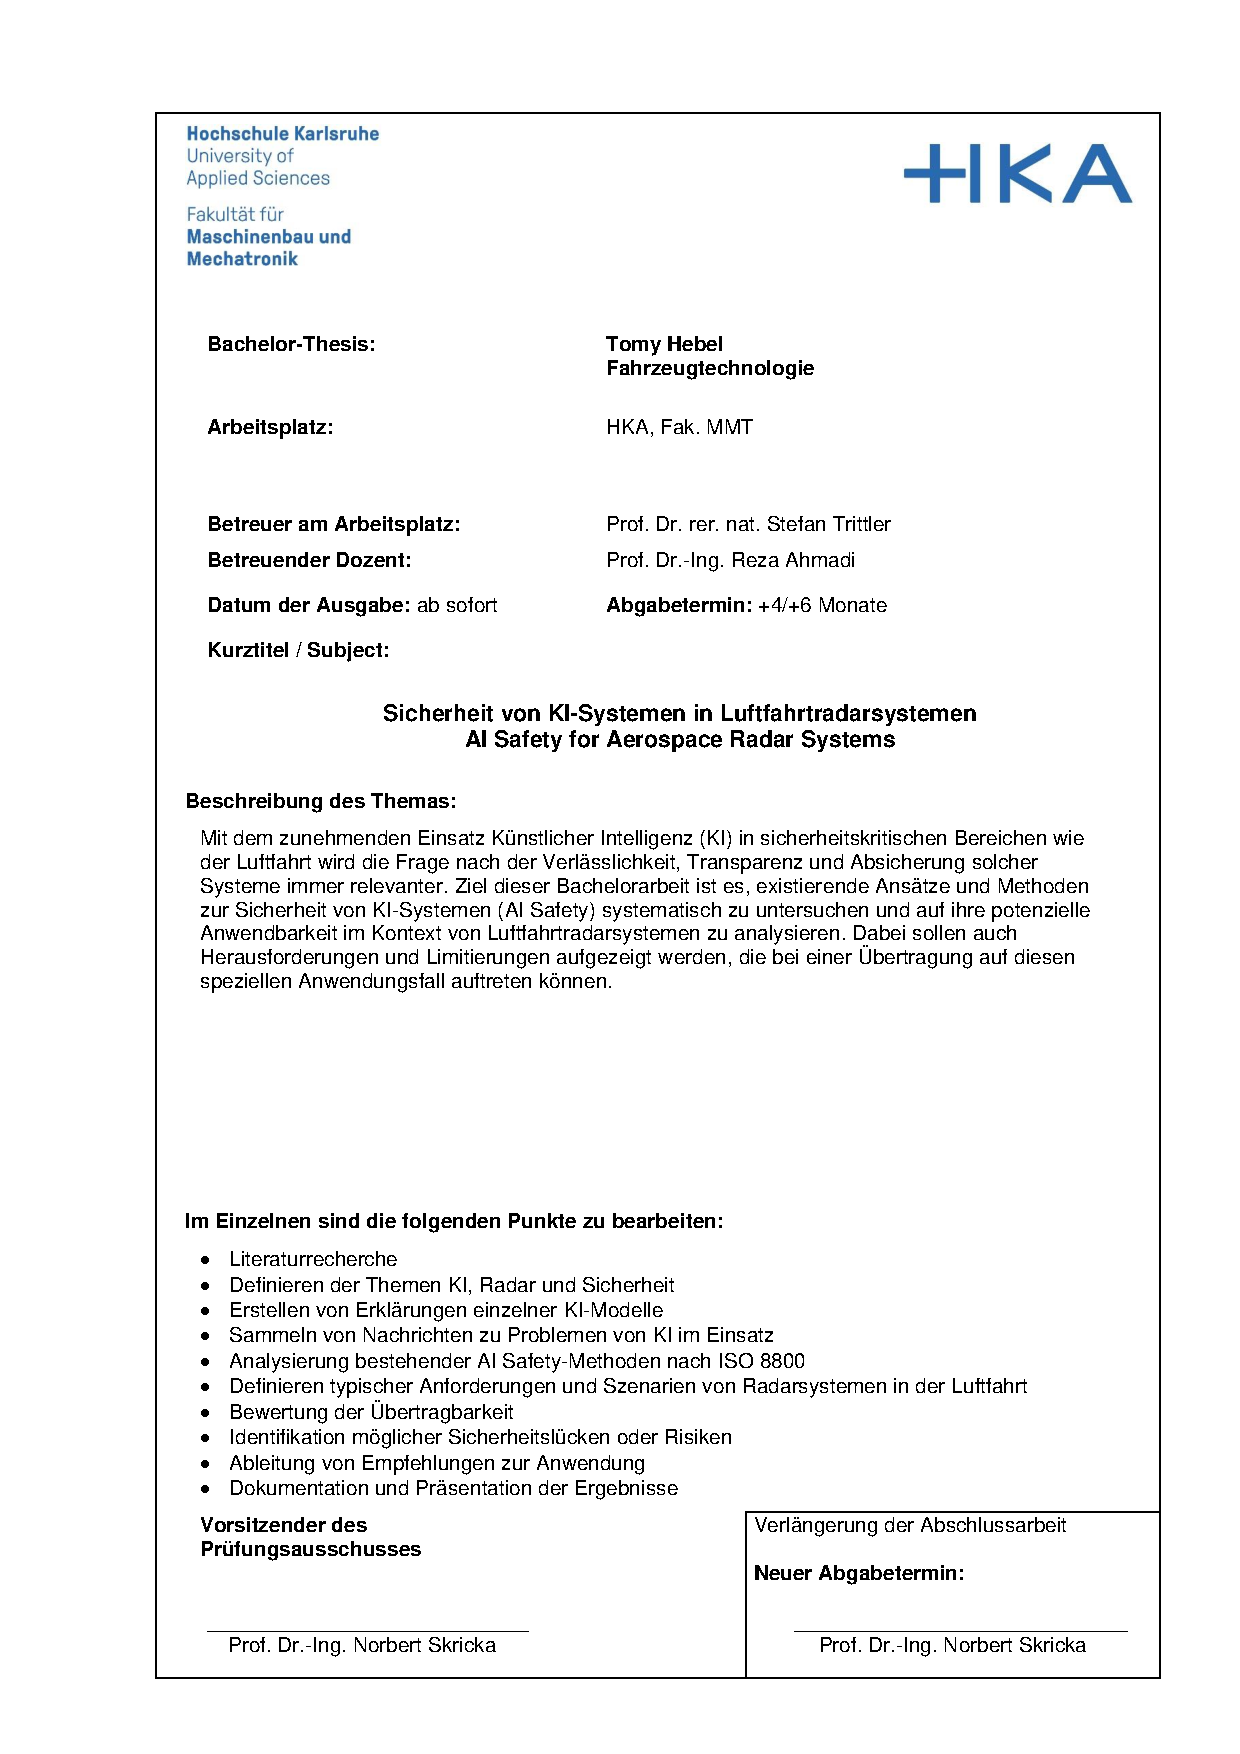
\includepdf[fitpaper=true, pages=-]{Bilder_und_Co/Sicherheit von KI-Systemen in Luftfahrtradarsystemen(1).pdf}

\chapter{Motivation und Ziel der Projektes}
Mit dem immer weiter verbreiteten Einsatz und Akzeptanz von \ac{KI} stellt sich die Frage, 
ob diese auch in der Luftfahrt Anwendung finden kann. Um diese Frage beantworten zu können, 
müssen \ac{KI} Modelle und ihr Eisatzgebiet auf Sicherheit überprüft werden. 

Ziel der Arbeit ist es, anhand des Beispieles von Radarsystemen zu überprüfen, 
ob KI-Systeme mittels bekannter Methodiken diese auf Sicherheit zu überprüfen ob sie den Anforderungen entsprechen, 
um diese in der Luftfahrt verwenden zu können.

\section{Weiteres}
In verschiedenen Paper wird gezeigt, dass \ac{KI} bei Radarsystemen was die Perfomance angeht, mit herkömmlichen Methoden 
mindestens mithalten kann oder diese was Rechenleistung, Speicher und Genauigkeit von Objekterkennung übertrifft. 
Dies unterstreicht weiter, dass es sehr nützlich sein kann \ac{KI} in diesem Feld zu benutzen. Doch in der Luftfahrt ist 
Sicherheit von großer Bedeutung und die meisten Paper die bei der Recherche zu diesem Thema gefunden wurden gehen 
auf die Performance der untersuchten KIs ein und untersuchen diese nicht auf Sicherheit, dies zeigt nochmals deutlich die Bedeutung 
dieser Arbeit. Doch was bedeutet sichere \ac{KI}? Ein Beispiel für eine Anforderung für eine sichere Software kann sein, 
dass diese deterministisch sein soll. Doch dies ist bezogen auf KIs problematisch umzusetzen, eine Möglichkeit wäre es, 
alle Möglichen Inputs und deren Outputs zu untersuchen bevor man die \ac{KI} verwendet. Aber das funktioniert nur bei 
kleieneren Modellen und würde vorallem bei Foundation Models einen zu großen Rechenaufwand bedeuten, als dass diese Methode 
verwendet werden könnte. Hier wäre eine persöhliche Idee einen Markowschen ansatz zu versuchen...??

\chapter{Hypothese}

\chapter{Methodisches Vorgehen}
\section{Besonders wichtige Literatur}
Zunächst wurde mit Absprache des Betreuenden Professors und dem Zweitkorrektor, eine kurze Liste an 
"Goldstandard-" Literatur festgelegt. Diese umfasst die recht neu erschienene ISO 8800 aus der Automobilbranche, 
welche die KI-Sicherheit in der Automobilbranche definiert. Die DO 178C weche über die Sicherheit von geschriebenen 
Computer Code in der Luftfahrt handelt. Und zum Schluss die EASA Roadmap und Concept Paper, welche beschreiben sollen, 
wie die Adaption von KI in der Luftfahrtbranche von statten gehen soll.


ISO 8800:

Diese ist die nach eigener Einschätzung, die derzeit Wertvollste Norm im Bezug auf KI-Sicherheit passend zum Kontext. 
Das liegt unteranderem an der Verwandschaft von der Luftfahrt und Automobilbranche, einerseitz technisch bzw. welche 
Ingenieurs-Fachgebiete abgedeckt werden, sowohl bei einem Flugzeug als auch bei einem Fahrzeug z.B. Aerodynamik, Elektrotechnik, 
Programmieren und vieles mehr. Die größeren Unterschiede hier liegen daher eher in den Anforderungen und Herangehensweisen 
im Bezug zur Sicherheit. Um beispielhafft einen sehr deutlichen Unterschied zu nennen, gibt es in der Automobilbranche 
die ISO 26262, die SOTIF Norm, welche sich mit der Sicherheit der Fuktionalität, unteranderem auch während des Betriebs 
des Fahrzeugs beschäftigt. Das kann zufolge haben, dass später im Lebenszyklus z.B. Softwareupdates erforderlich sind. 
Im Gegensatz wird in der Luftfahrt dieses Thema hauptsächlich im Frontloading behandelt, unter der Prämisse, dass das Flugzeug 
bereits bei erstigem Einsatz alle Sicherheitsanforderungen zur Gänze erfüllt und spätere Softwareupdates obsulet macht oder 
vorher definiert wird was und wann geändert werden muss mittels Updates.

Des Weiteren ähneln sich beide Branchen im Bezug auf die Sicherheit einzelner Komponenten. Z.B. werden in der Automobilbranche 
sehr hohe Sicherheitsanforderungen für einzelne Komponenten definiert, damit diese nicht redundant verbaut werden müssen und somit 
der Stückpreis pro Fahrzeug steigt, da bei Großserien redundante Teile sehr teuer sind. Hingegen wird in der Luftfahrt 
allgemein sehr hohe Ansprüche an alle einzelnen Teile gelegt, da die Gefahr bei Fehlfunktionen in einem Flugzeug sehr schnell 
lebensbedrohlich wird. Um weitere Sicherheit zu gewährleisten und um die definierten Anforderungen zu erfüllen werden die 
Teile in einem Flugzeug redundant verbaut.

Weitere Technische Unterschiede der Branchen gehen aus ihrer Natur herfor. In der Automobilbranche wird sehr viel B2C gehandelt, 
während die Luftfahrt hauptsächlich B2B handelt. Aufgrund der im Vergleich geringeren Lebensbedrohlichkeit bei Fehlfunktionen 
und der Branchennatur private Kunden zu gewinnen, befasst sich die Automobilbranche unteranderem viel mit technischen Begeisterungsmerkmahlen. 
Die Luftfahrt verfolgt das Ziel Geschäftskunden zu gewinnen, welche andere Wünsche haben als Privatpersonen.
Auf Grund dieses Unterschiedes kann sich die Automobilbranche sehr früh mit neueren Technologien auseinandersetzen, wo hingegen die 
Luftfahrt sich intensiv mit der Notwendigkeit und Sicherheit dieser neuen Technologien befasst. Weiter zu betrachten ist der gesammte Produktlebenszyklus, 
da Flugzeuge ca. zweimal so lange im Gebrauch sind wie Autos, was das Thema Sicherheit verkompliziert, besonders unter der Berücksichtigung 
von sich verändernde Umgebungen. (Beispiele hierfür sind im Straßenverkehr in den letzten Jahren eine größere Verbreitung von 
Elektrorollern zu beobachten. Und in der Luftfahrt nimmt der Einsatz von Dronen zu.)Z.B. kann die Automobilbranche mit einer KI 
gesteuerten Schilderkennung Kundengewinnen und Erfahrungen sammeln, während in der Luffahrt Wolken und Wetter Erkennung mit einer 
KI die Evaluierung und Entwicklung langwieriger ist. Das und noch mehr Gründe erklären, warum 
es die Luftfahrbranche daher technologisch träger macht. Aufgrund dieser Natur und der technischen Verwandheit wäre es sinnvoll, 
dass die Luftfahrt von den Erfahrungen der Automobilbranche lernen kann.


DO 178C:

Diese Luftfahrt Norm befasst sich mit der Sicherheit von geschrieben Computercode, zu erwähnen sind die Normen, auf die Bezug genommen werden in der 
DO 178C. Z.B. die DO 330 und die DO 333, welche sich mit Sofwarewerzeugen und deren Zertifizierung beschäftigen. Um den Aufwand nicht in das Unermessliche 
zu treiben werden diese nur bei bedarf angeschnitten. Da KI in verschiedener Literatur beschrieben "(z.b. ISO 5469TR)" als mathematischer 
Algorithmus und Teil der Softeware behandelt werden kann/sollte muss KI auch in Einklang gebracht werden mit der DO 178C. Was hier besonders interessant 
ist, sind bestimmte Anforderungen an Computer Code. Z.B. das der Code deterministisch sein soll und eine MC/DC coverage. Das KI oftmals nicht deterministisch 
ist, ist Allgemeinwissen. "(Unter bestimmten Vorraussetzungen kann KI deterministisch sein, z.B. wenn man die Temperatur des Outputvektors in einem NN auf 0 setzt 
und man den gesammten Inputraum abgedeckt/getestet hat. Doch das ist meistens technisch nicht umsetzbar oder würde die Funktion/Fähigkeit der KI zusehr einschränken)" 
MC/DC coverage beschreibt, dass jede einzelne Bedingung bei Entscheidungen z.B. if/else Schleifen im Code auch stehts ein anderen Output erzeugt. 
Das eine KI diese Anforderung nicht erfüllen kann sollte ebenfalls recht offensichtlich sein. Doch das interessante ist, dass in der 
DO 178C das nur implizit und nicht explizit gefordert wird. Um etwas genauer zu werden, werden diese Anforderungen sowohl in der DO 178C als auch 330 und 333 sehr 
empfohlen und als "best practise" beschrieben.


EASA AI Roadmap:

Die EASA ist die Europäische Agentur für Flugsicherheit. Die Regularien der EASA werden weltweit als "best practise" Standards anerkannt.
Und um Produkte in der europäischen Luftfahrtbranche anbieten zu können, müssen Flugzeughersteller EASA-Zulassungen besitzen. 
Auf Grund dieser Bedeutung und des Wissens und Erfahrungen der Sicherheitsingenieure dieser Agentur, muss nicht weiter 
ausgeführt werden, warum diese veröffentlichten Konzepte hier mit besonderer Bedeutung berücksichtigt wurden.
Doch leider sind die Veröffentlichten Konzepte leider nicht mehr als genau das. In diesen Konzepten stehen 
viele "best practise" Methoden und zu berücksichtigende Punkte, jedoch leider nicht, wie bei einer Norm, 
dass wenn alle dieser Punkte erfüllt sind, dass das Produkt sicher ist. Hier ein kleiner Spoiler vorab, sehr viele dieser Punkte 
und Methoden sind deckungsgleich mit dem was in der ISO 8800 steht. Die ISO 8800 geht konkreter auf Anpassungen 
zu berücksichtigender Normen ein und beschreibt ins Detail was wie Dokumentiert werden muss. "(Weiteres später)"

\section{Recherche}
Der zweite Schritt war weitere Literaturrecherche. Für die vorliegende Recherche wurden verschiedene wissenschaftliche Quellen systematisch ausgewertet. 
Dabei kamen unter anderem etablierte Datenbanken wie Google Scholar, ProQuest und IEEE Xplore zum Einsatz. 
Zur Sicherstellung einer umfassenden Betrachtung des Themas wurde die Auswahl der Quellen jedoch nicht 
ausschließlich auf diese Datenbanken beschränkt, sondern durch weitere spezialisierte Plattformen und 
einschlägige Fachpublikationen ergänzt. Ziel war es, eine breite und ausgewogene Grundlage für die Analyse 
und Darstellung der Thematik zu schaffen. Zudem war das Vorgehen zuerst anhand des Titels eine Thematische 
Verwandschaft festzustellen. Wenn im Titel kein Hinweis auf eines der Subthemen: KI, Radarsysteme, Luftfahrt 
oder Sicherheit zu erkennen war, wurden die Wissenschaftlichen Paper nicht weiter evaluiert. Die Paper, 
die ein Hinweis auf mindestens eines dieser Subthemen aufwieß wurde es Systematisch festgehalten und anhand 
des Abstractes auf tiefergehende Relevanz untersucht. Wenn das Abstract weitere Thematische Zusammenhänge 
gezeigt hat, wurde es berücksichtigt. Probleme die hier öfter aufgetreten sind waren, dass im Kontext KI 
es sich oftmals um Performance Paper gehandelt hat. Diese Performance Paper folgten meist dem Schema zu erklären, 
wie, warum und wofür diese KI trainiert wurde und ihre Fähigkeiten aufgezeigt. Diese Paper hatten zwei Probleme, 
einerseits waren sie nicht besonders relevant für das Thema und eine relative Performance im Vergleich zu 
herkömmlichen Methoden wurde meist auch nicht ausgeführt.


\chapter{Aufbau der Arbeit} 
\part{Grundlagen und Kontext}
\chapterimage{Bilder_und_Co/a_magnifying_glass_which_points_out_a_neuronal_network_surrounded_by_computer_code_and_a_question_ma_296098326.png} % Chapter heading image
%----------------------------------------------------------------------------------------
\chapter{Radar in der Luftfahrt}

\usetikzlibrary{arrows.meta, positioning}

\section{Radar – Grundlagen (allgemein)}

\subsection{Prinzip}
Ein Radar sendet elektromagnetische Wellen aus und misst Laufzeit,
Frequenzverschiebung und Einfallswinkel der Echos.
Daraus folgen Entfernung, Geschwindigkeit und Winkel der detektierten Objekte.
\begin{itemize}
  \item Laufzeit $\Rightarrow$ Entfernung
  \item Doppler $\Rightarrow$ Relativgeschwindigkeit
  \item Antenne/Beam $\Rightarrow$ Winkel
\end{itemize}

\subsection{Systemklassen und Betriebsarten}
\begin{itemize}
  \item \textbf{Mono-/Bi-/Multistatisch}: Unterscheidung danach, ob Sende- und Empfangsort identisch sind
        (monostatisch, in der Luftfahrt dominierend) oder räumlich getrennt (bi-/multistatisch).
  \item \textbf{Wellenformen}:
    \begin{itemize}
      \item \textbf{Gepulst / Puls-Doppler} $\Rightarrow$ Standard für Entfernungsbestimmung (z.\,B. Primärradar zur Luftraumüberwachung am Boden)
            und bei vielen Bordradaren; Puls-Doppler nutzt zusätzlich die Frequenzverschiebung.
      \item \textbf{Kontinuierlich (CW)} $\Rightarrow$ misst primär Geschwindigkeit; ohne Modulation keine Entfernung.
      \item \textbf{Frequenzmoduliert (FMCW)} $\Rightarrow$ weit verbreitet bei Radarhöhenmessern und zunehmend bei Drohnen
            oder in der Fahrzeugtechnik (Kurz-/Mittelreichweite).
    \end{itemize}
  \item \textbf{Scanprinzip}:
    \begin{itemize}
      \item \textbf{Mechanisch geschwenkt} $\Rightarrow$ Standard bei klassischen Primärradaren oder älteren Bordradaren.
      \item \textbf{Elektronisch geschwenkt} $\Rightarrow$ mehrkanalig für präzisere Winkelmessung,
            zunehmend bei modernen Wetterradaren und im militärischen Bereich.
    \end{itemize}
\end{itemize}

\subsection{Luftfahrtkontext}
\begin{itemize}
  \item \textbf{Bodenradar}: Primärradar (PSR) zur Detektion nicht-kooperativer Ziele;
        Sekundärradar (SSR/Mode A/C/S) für kooperative Abfrage. (Bei einer Kooperativen Anfrage wird das Radar zur Kommunikation genutzt)
  \item \textbf{Bordradar}: Wetterradar (WXR) zur Gewitter- und Niederschlagserkennung; Umfeld für Kollisionswarnsysteme.
  \item \textbf{Radarhöhenmesser}: FMCW-basiert, liefert die Höhe über Grund für Anflug/Landung und Systemlogik.
\end{itemize}

\subsection{Störquellen und Szenarien}
Radare heb viele mögliche Störquellen und Szenarien, die die Effektivität einschränken können.
Einige Beispiele sind:
\begin{itemize}
  \item \textbf{Thermisches Rauschen}: Fundamentales Hintergrundrauschen der Empfangselektronik; begrenzt die minimale detektierbare Signalstärke.
  \item \textbf{RFI (Radio Frequency Interference)}: Störungen durch andere Funksender oder Systeme (z.\,B. Kommunikationsfunk, Navigationshilfen, benachbarte Radare).
  \item \textbf{Mehrwegeausbreitung (Multipath)}: Reflexionen am Boden oder an Strukturen führen zu Mehrwege-Signalen, die Phasenfehler und Geisterziele verursachen können.
  \item \textbf{Clutter (Boden, See, Wetter)}: Starke Reflexionen stationärer Flächen erschweren die Detektion bewegter Ziele.
  \item \textbf{Regen / Dämpfung (Attenuation)}: Besonders in höheren Frequenzbändern relevant; starke Niederschläge dämpfen das Signal und erzeugen zusätzlichen Clutter.
  \item \textbf{Jamming / Deception}: Überlagerung des Empfangssignals mit breitbandigem Rauschen oder absichtliche Erzeugung falscher Ziele (z.\,B. per DRFM), um das Radarsystem zu stören.
  \item \textbf{Zielschwankungen}: Die Reflektionsstärke (Radar Cross Section, RCS) schwankt abhängig von Geometrie, Material und Ausrichtung des Ziels.
  \item \textbf{Interferenzen durch kooperative Systeme}: Sekundärradar- und ADS-B-Signale können sich überlagern und Störungen erzeugen.
  \item \textbf{Atmosphärische Effekte}: Brechung, Duktung oder Turbulenzen verändern die Ausbreitung und können scheinbare Zielbewegungen hervorrufen.
\end{itemize}

\subsection{Signalverarbeitungskette}
\usetikzlibrary{arrows.meta, positioning}
\tikzset{
  block/.style = {rectangle, draw, rounded corners, minimum width=5cm, minimum height=1cm, align=center},
  arrow/.style = {thick, -{Stealth[]}},
  explain/.style = {align=left, text width=8cm}
}

\begin{tikzpicture}[node distance=1.5cm]
  % Hauptkette
  \node[block] (raw) {1) Rohdaten};
  \node[explain, right=1cm of raw] {Basisbandsignale (I/Q-Samples) direkt vom Radar-Frontend. Ausgangspunkt aller weiteren Schritte.};

  \node[block, below=of raw] (range) {2) Pulskompression / Range-FFT};
  \node[explain, right=1cm of range] {Erhöht die Empfindlichkeit und liefert eine feinere Entfernungsauflösung mittels Matched Filtering oder Range-FFT.};

  \node[block, below=of range] (doppler) {3) Doppler-FFT über Pulse};
  \node[explain, right=1cm of doppler] {Auswertung der Frequenzverschiebung über die Pulsfolge. Liefert die Radialgeschwindigkeit bewegter Ziele.};

  \node[block, below=of doppler] (rdmap) {4) Range–Doppler-Map (RD)};
  \node[explain, right=1cm of rdmap] {Zweidimensionale Darstellung mit Achsen Entfernung und Geschwindigkeit; Grundlage für Detektion und Klassifikation.};

  \node[block, below=of rdmap] (cfar) {5) CFAR / Maskierung};
  \node[explain, right=1cm of cfar] {Adaptive Schwellwertbildung mit lokaler Störschätzung. Hält die Falschalarmrate konstant und unterdrückt Clutter.};

  \node[block, below=of cfar] (cluster) {6) Clustering};
  \node[explain, right=1cm of cluster] {Gruppiert benachbarte Detektionen zu kohärenten Objekten, z.\,B. zu einem Flugzeugziel.};

  \node[block, below=of cluster] (track) {7) Tracking (Kalman)};
  \node[explain, right=1cm of track] {Verfolgt Objekte über die Zeit, glättet Messrauschen und löst Mehrziel-Konflikte. Grundlage für stabile Trajektorien.};

  \node[block, below=of track] (hmi) {8) HMI / Interfaces};
  \node[explain, right=1cm of hmi] {Visualisierung (z.\,B. Wetterradar-Anzeige) und Übergabe an Avioniksysteme zur weiteren Nutzung.};

  % Verbindungen Hauptkette
  \draw[arrow] (raw) -- (range);
  \draw[arrow] (range) -- (doppler);
  \draw[arrow] (doppler) -- (rdmap);
  \draw[arrow] (rdmap) -- (cfar);
  \draw[arrow] (cfar) -- (cluster);
  \draw[arrow] (cluster) -- (track);
  \draw[arrow] (track) -- (hmi);
\end{tikzpicture}

\subsection{Detektion \& CFAR (Constant False Alarm Rate)}
Ein Radar empfängt neben echten Zielen immer auch Rauschen, Clutter und Störsignale.
Daher muss entschieden werden, ob das Echo ein echtes Ziel oder nur Zufall bzw.\ Clutter ist.
Bei zu niedrigem Schwellenwert steigen zwar die Treffer, aber auch die Fehlalarme;
bei zu hohem Schwellenwert sinken Fehlalarme, schwache Ziele gehen verloren.

\subsection{Auflösungen und Messfehler}
\begin{itemize}
  \item \textbf{Entfernungsauflösung}: Wie nahe zwei Ziele in Reichweite beieinanderliegen dürfen, um getrennt zu erscheinen;
        bestimmt durch Puls- und Signalbandbreite.
  \item \textbf{Geschwindigkeitsauflösung}: Kleinste unterscheidbare Relativgeschwindigkeit; geprägt durch Beobachtungszeit
        und Anzahl der ausgewerteten Pulse.
  \item \textbf{Winkelauflösung}: Fähigkeit, Ziele im Azimut oder in der Elevation zu trennen; abhängig von Antennenapertur und Verfahren der Winkelschätzung.
  \item \textbf{Reichweitenmessfehler}: Zufällige Abweichungen der gemessenen Entfernung; beeinflusst durch SNR und Pulskompression.
  \item \textbf{Geschwindigkeitsmessfehler}: Unsicherheit in der Doppler-Schätzung; abhängig von SNR (Signal-Rausch-Verhältnis), Beobachtungsdauer und Senderstabilität.
  \item \textbf{Winkelmessfehler}: Abweichung zwischen gemessenem und tatsächlichem Zielwinkel; abhängig von SNR, Antennengröße und Verfahren.
\end{itemize}

\subsection{Typische Trade-offs}
\begin{tabular}{p{0.3\textwidth} p{0.65\textwidth}}
\textbf{Reichweite vs.\ Auflösung} & Mehr Bandbreite verbessert die Entfernungsauflösung, erhöht aber Rauschbandbreite, Datenrate und Systemkomplexität. \\[0.5em]
\textbf{CPI-Länge} & Längere Beobachtung verbessert Dopplerauflösung und Empfindlichkeit, erhöht aber Latenz und kann bei stark manövrierenden Zielen zu Unschärfe führen. \\[0.5em]
\textbf{Zeit–Frequenz–Unschärfe} & Oder Heisenbergsche Unschärferelation: Kurze Signale lokalisieren ein oder mehrere Ziele gut (gut für Reichweite), verlieren aber Frequenzpräzision (schlechter um die Geschwindigkeit von Zielen zu bestimmen); lange Signale umgekehrt. \\[0.5em]
\textbf{Detektionsschwelle vs.\ Fehlalarme} & Niedriger Schwellenwert steigert die Entdeckungswahrscheinlichkeit, aber auch die Falschalarmrate; höherer Schwellenwert reduziert Fehlalarme, kann schwache Ziele verpassen. CFAR gleicht dies adaptiv aus. \\[0.5em]
\textbf{Clutter-Unterdrückung vs.\ Zielerhalt} & Aggressive Filterung (z.\,B.\ MTI, Wettermasken) reduziert Störungen, riskiert aber langsame oder schwache Ziele zu dämpfen. \\[0.5em]
\textbf{Datenrate/Kompression vs.\ Informationsgehalt} & Hohe Abtastraten, viele Kanäle und feine Raster liefern reichhaltige RD(A)-Daten, treiben aber Schnittstellenlast, Speicher und Latenz. Kompression/Dezimierung spart Ressourcen, verliert aber Details. \\[0.5em]
\textbf{Wellenform-Komplexität vs.\ Robustheit} & Komplexe, modulierte Wellenformen bieten bessere Auflösung und Anti-Jam-Eigenschaften, erhöhen aber Implementierungsaufwand und Empfindlichkeit gegenüber Modellfehlern. \\[0.5em]
\textbf{Abdeckungsrate vs.\ Verweilzeit} & Schnelles Scannen erhöht Volumenabdeckung und Aktualität, reduziert jedoch Verweilzeit pro Blickrichtung und damit SNR; längere Verweilzeiten erhöhen SNR, senken aber Abdeckungsrate. \\
\end{tabular}

\subsection{Leistungskennzahlen (System \& Messung)}
\begin{tabular}{p{0.3\textwidth} p{0.65\textwidth}}
\textbf{Entdeckungswahrscheinlichkeit (Pd)} & Wahrscheinlichkeit, dass ein tatsächlich vorhandenes Ziel erkannt wird; hoher Wert bedeutet zuverlässige Detektion. \\[0.5em]
\textbf{Falschalarmwahrscheinlichkeit (Pfa)} & Wahrscheinlichkeit, dass ein Ziel gemeldet wird, obwohl keines existiert (z.\,B.\ durch Rauschen oder Clutter). \\[0.5em]
\textbf{ROC-Kurve} & Zeigt den Zusammenhang zwischen Pd und Pfa; macht den Trade-off sichtbar. \\[0.5em]
\textbf{Messfehler (Range, Geschwindigkeit, Winkel)} & Zufällige Abweichungen zwischen gemessenen und wahren Werten; beeinflusst durch SNR, Integrationszeit und Systemstabilität. \\[0.5em]
\textbf{Update-Rate / Latenz} & Zeitliche Aktualisierung der Messungen; höhere Raten verbessern Situationsbewusstsein, können jedoch die Verweilzeit reduzieren. \\[0.5em]
\textbf{Verfügbarkeit / Zuverlässigkeit} & Fähigkeit des Systems, über lange Zeit stabil Daten zu liefern – trotz Störungen oder widriger Bedingungen. \\
\end{tabular}


\section{Radar – Grundlagen für Objektklassifizierung}

\subsection{Wichtige Datenpunkte für Objektklassifikation}
\begin{tabular}{p{0.35\textwidth} p{0.6\textwidth}}
\textbf{Reichweite (Entfernung)} & Basisinformation für die Position eines Objekts relativ zum Radar; zentral für Lagebestimmung und Tracking. \\[0.5em]
\textbf{Relativgeschwindigkeit (Doppler)} & Erkennt Bewegung auf das Radar zu oder davon weg. Wichtig, um bewegte von statischen Objekten zu unterscheiden. \\[0.5em]
\textbf{Winkel (Azimut/Elevation)} & Richtung, aus der das Echo kommt. Unerlässlich für räumliche Lokalisierung und die Trennung mehrerer Ziele. \\[0.5em]
\textbf{Radar Cross Section (RCS)} & Stärke der Reflexion, abhängig von Größe, Material und Geometrie des Objekts; hilfreich für Typ- und Größenindizien. \\[0.5em]
\textbf{Doppler-Signatur / Mikrodoppler} & Feinstruktur durch bewegte Teile (z.\,B.\ Rotorblätter, Flügelschlag); liefert starke Trennmerkmale. \\[0.5em]
\textbf{Zeitliche Historie / Tracks} & Trajektorien über mehrere Messzyklen machen Verhalten sichtbar (z.\,B.\ stabile Flugbahn vs.\ flatternde Bewegung). \\[0.5em]
\textbf{Spektrale Eigenschaften der Echos} & Verteilung der Rückstreuung über Frequenz oder Polarisation kann Material- und Strukturhinweise geben. \\[0.5em]
\textbf{Clutter-Kontext} & Einordnung des Objekts im Umfeld: Bodenclutter, Wetter oder Seeoberfläche beeinflussen die Klassifikationssicherheit. \\[0.5em]
\textbf{SNR und Qualitätsmetriken} & Signal-Rausch-Verhältnis, CFAR-Maske, lokale Störschätzung; entscheidend, um unsichere Messungen korrekt zu gewichten. \\[0.5em]
\textbf{Sensor-/Modus-Metadaten} & Hinweise zu Wellenform, PRF, Antennen-Aspect oder Scanmodus helfen, Merkmale richtig zu interpretieren. \\[0.5em]
\textbf{Konsistenz über Zeit} & Persistenz, Aussetzer, Track-Confidence und Plausibilitätschecks (kinematische Grenzen) erhöhen die Robustheit. \\
\end{tabular}

\section{Merksätze zu Radar-Grundlagen und Objektklassifizierung}

\subsection{Radar-Grundlagen – wichtigste Merksätze}
\begin{itemize}
  \item \textbf{Physik zuerst:} Das Signal-Rausch-Verhältnis setzt die Grenzen – alles Weitere baut darauf auf.
  \item \textbf{Qualität wandert nach unten:} Stabilität von Range–Doppler–Angle bestimmt die Qualität aller Folgeschritte.
  \item \textbf{PRF ist ein Hebel:} Wahl der Pulsfolge legt den Kompromiss zwischen Reichweite und Geschwindigkeitsmessung fest.
  \item \textbf{Bandbreite kostet:} Bessere Auflösung erhöht Datenrate, Rechenlast und Anforderungen an Hardware.
  \item \textbf{Antenne = Winkel:} Größere Apertur oder elektronisches Schwenken verbessert Winkeltrennung, aber treibt Komplexität und Energiebedarf.
  \item \textbf{Beobachtungszeit vs.\ Latenz:} Längere Integrationszeiten schärfen Doppler, erhöhen aber Latenz und Bewegungsunschärfe.
  \item \textbf{CFAR steuert Falschalarmrate:} Zu niedrige Schwellen erzeugen Fehlalarme, zu hohe verpassen schwache Ziele.
  \item \textbf{Clutter ist der Hauptgegner:} Filter aggressiv genug wählen, ohne langsame oder schwache Ziele zu unterdrücken.
  \item \textbf{Mehrwege und Atmosphäre machen Geister:} Tracking und Konsistenzprüfungen enttarnen Scheinziele.
  \item \textbf{Koexistenz beachten:} Betrieb neben SSR/ADS-B, Funk- und Navigationsdiensten erfordert robuste Störfestigkeit.
  \item \textbf{Kalibrierung hält Systeme ehrlich:} Regelmäßige Checks und Health-Monitoring sichern Vergleichbarkeit und verhindern Drift.
  \item \textbf{Metadaten sind Gold:} Modus-, PRF- und Antenneninformationen gehören in die Daten, damit Auswertungen interpretierbar bleiben.
\end{itemize}

\subsection{Objektklassifizierung – wichtigste Merksätze}
\begin{itemize}
  \item \textbf{Stabilität vor KI:} Saubere Detektion, verlässliche RD/RDA-Daten und stabile Tracks sind die Basis guter Klassifikation.
  \item \textbf{Zeit schlägt Einzelbild:} Sequenzen und Trajektorien glätten Rauschen und offenbaren Muster besser als Einzelscans.
  \item \textbf{Mikrodoppler als Fingerabdruck:} Rotor- und Flügelschlag-Signaturen trennen Drohnen, Helikopter und Vögel – abhängig von SNR und Aspekt.
  \item \textbf{Quality-in-the-loop:} SNR, CFAR-Masken, Clutter- und Jamming-Flags als zusätzliche Eingabekanäle erhöhen Robustheit.
  \item \textbf{Offene Welt akzeptieren:} Eine \emph{Unknown}-Option und OOD-Detektion sind Pflicht – lieber aussetzen als falsch sicher sein.
  \item \textbf{Konfidenz muss stimmen:} Kalibrierte Wahrscheinlichkeiten und klare Abstain-Schwellen sind wichtiger als maximale Top-1-Quote.
  \item \textbf{Physik hilft:} Physikgeleitete Merkmale (z.\,B.\ kinematische Plausibilität, Spektralbreite, RCS-Trends) stabilisieren datengetriebene Modelle.
  \item \textbf{Szenariodeckung vor „Overall-Accuracy“:} Leistung immer nach SNR, Entfernung, Aspekt und Umgebung berichten – sonst täuscht Mittelung.
  \item \textbf{Splits ohne Leckage:} Trainings-/Testtrennung nach Szenarien (Standorte, Aspekte, Wetterlagen) verhindert zu optimistische Ergebnisse.
  \item \textbf{HMI klärt Erwartungen:} Anzeige von Top-k, Konfidenz und OOD/Qualitätsflags verhindert Fehlinterpretationen im Betrieb.
  \item \textbf{Vorverarbeitung prägt Merkmale:} Wahl von CFAR, Filterung und Normalisierung bestimmt, was das Modell überhaupt „sehen“ kann.
  \item \textbf{Robust denken:} Klassifikation muss mit Clutter, RFI und sporadischen Aussetzern umgehen – Fallbacks gehören zum Design.
\end{itemize}








\chapter{Sicherheit in der Luftfahrt}
\textbf{Sicherheit verstehen bedeutet, Risiken zu verstehen.}\\
Sicherheit (Safety) ist die Freiheit von unvertretbaren Risiken; Risiko bemisst sich über Eintrittswahrscheinlichkeit und Schadensschwere.

\section{Sicherheit – Grundlagen}

\subsection{Begriffsabgrenzung: Safety vs. Security}
Safety = Schutz vor unbeabsichtigten Fehlern/Versagen. \\
Security = Schutz vor absichtlichen Angriffen.\\

\subsection{Risikobegriffe und Schutzziele}
Risiko beschreibt die Kombination aus \emph{Schweregrad} einer möglichen Auswirkung und ihrer \emph{Eintrittswahrscheinlichkeit}. 
Beide werden gemeinsam (z.\,B. in einer Risikomatrix) bewertet, um ein \emph{tolerierbares Restrisiko} festzulegen. 
Ziel ist, Risiken durch geeignete Maßnahmen so weit zu mindern, dass sie akzeptabel sind (ALARP-Prinzip: as low as reasonably practicable).

\paragraph{Schutzziele (Safety Goals).}
Aus der Bewertung werden klare Schutzziele abgeleitet: Sie beschreiben, welche gefährlichen Zustände verhindert bzw.\ auf welche Weise sie beherrscht werden müssen (z.\,B.\ definierte Fallback-Zustände, Grenzen für Fehlalarme und Ausfälle).

\paragraph{Abgeleitete Sicherheitsanforderungen.}
Die Schutzziele werden in überprüfbare Anforderungen überführt (z.\,B.\ Reaktionszeiten, Verfügbarkeiten, Fehlertoleranz). 
Diese Anforderungen sind rückverfolgbar zu den identifizierten Risiken und bilden die Grundlage für Verifikation und Validierung.

\paragraph{Risikominderungsmaßnahmen.}
Maßnahmen lassen sich typischerweise in drei Kategorien gliedern:
\begin{itemize}
  \item \textbf{Präventiv} (Fehler vermeiden): robuste Architektur, Redundanz, Partitionierung.
  \item \textbf{Detektierend} (Fehler erkennen): Überwachung, Plausibilitätsprüfungen, Alarme.
  \item \textbf{Korrektiv} (Fehler beherrschen): Fallbackmodus, sichere Abschaltung. 
\end{itemize}

\paragraph{Akzeptanzkriterien und Nachweis.}
Akzeptanzkriterien definieren, wann ein Restrisiko als tragbar gilt. Die Erfüllung wird durch Analysen, Tests und Inspektionen nachgewiesen und über den gesamten Lebenszyklus dokumentiert (Traceability von Gefährdung $\rightarrow$ Schutzziel $\rightarrow$ Anforderung $\rightarrow$ Nachweis).
Das ist essentiell für die Entwicklung von Komponenten und muss angemssen Dokumentiert werden in der Safety-Argumentation.

\subsection{Safety-Argumentation (Assurance Case)}
Ein \emph{Assurance Case} begründet systematisch und nachvollziehbar, dass ein System unter definierten Einsatzbedingungen \emph{sicher genug} ist. 
Er verbindet nachvollziehbare Behauptungen (Claims/Goals) mit einer transparenten Argumentationsstruktur, dokumentierten Annahmen und geeigneten Nachweisen (Analysen, Tests).

\paragraph{Zweck und Grundprinzip.}
Ziel ist eine prüfbare Argumentation: 
\begin{itemize}
    \item \emph{Was} wird behauptet (Claim)
    \item \emph{warum} ist das plausibel (Strategie/Begründung)
    \item \emph{unter welchen Bedingungen} gilt es (Kontext/Annahmen)
    \item \emph{wodurch} wird es gestützt (Evidenz)
\end{itemize}
Die Argumentation ist der Kern der Dokumentation und dient als Nachweis das etwas sicher genug ist.

\subsection{Gefahrenanalyse und Risikoermittlung}
Ziel der Gefahrenanalyse ist es, mögliche Gefährdungen früh zu erkennen, ihr Risiko grob einzuordnen und wirksame Gegenmaßnahmen abzuleiten. Das Ergebnis ist eine priorisierte Liste von Risiken mit klaren Safety-Zielen und abgeleiteten Anforderungen – und ein Plan, wie diese nachgewiesen werden.

\paragraph{Ablauf in Kurzform.}
\begin{enumerate}
  \item \textbf{Sammeln:} Mögliche Gefährdungen identifizieren (Technik, Mensch, Umfeld, Betrieb).
  \item \textbf{Einordnen:} Schweregrad und Eintrittswahrscheinlichkeit bewerten (Risikomatrix).
  \item \textbf{Maßnahmen ableiten:} Präventiv, detektierend, korrektiv.
  \item \textbf{Anforderungen festlegen:} Messbar, überprüfbar, rückverfolgbar.
  \item \textbf{Pflegen:} Über den Lebenszyklus regelmäßig aktualisieren.
\end{enumerate}

\paragraph{Methoden (kurz erklärt).}
\begin{itemize}
  \item \textbf{Hazard Identification (HAZID):} Strukturierte Sammlung von Gefährdungen per Workshops, Checklisten und Erfahrungswissen. Ergebnis: Hazard-Liste mit Ursachen, Wirkungen und Annahmen.
  \item \textbf{FMEA/FMECA:} \emph{Bottom-up} auf Komponenten- oder Funktionsebene: Welche Ausfallarten gibt es, was passiert dann, wie wird es entdeckt? FMECA ergänzt eine Kritikalitätsbewertung, um Prioritäten zu setzen.
  \item \textbf{Fault Tree Analysis (FTA):} \emph{Top-down} vom unerwünschten Ereignis (z.\,B. Verlust der Warnfunktion) zu seinen Ursachen. Eignet sich, Ketten/Wechselwirkungen sichtbar zu machen.
  \item \textbf{STPA:} Systemtheoretischer Ansatz: Welche \emph{unsicheren Steueraktionen} und Rahmenbedingungen führen zu Gefährdungen – inkl.\ Software, HMI und Prozeduren, nicht nur Hardware.
\end{itemize}

\subsection{Architekturprinzipien der funktionalen Sicherheit}
Ziel dieser Prinzipien ist es, Risiken durch die Systemarchitektur zu senken: Fehler sollen gar nicht erst wirken, früh erkannt oder sicher beherrscht werden. Im Fokus stehen klare Strukturen, vorhersehbares Verhalten und beherrschte Degradation statt Überraschungen.

\paragraph{Redundanz und Diversität/Dissimilarität}
\textbf{Redundanz} bedeutet, kritische Funktionen mehrfach vorzuhalten (z.\,B.\ zwei unabhängige Empfangsketten oder Stromversorgungen), sodass beim Ausfall einer Instanz die andere übernimmt.
\textbf{Diversität/Dissimilarität} ergänzt dies durch bewusst unterschiedliche Ausprägungen (z.\,B.\ verschiedene Hardware/Software oder unterschiedliche Algorithmen), damit ein gemeinsamer Fehler nicht alle Kanäle gleichzeitig trifft.
\emph{Beispiel:} Zwei unabhängige Radarpfade, davon einer mit alternativer Signalverarbeitung.

\paragraph{Trennung/Partitionierung}
Trennung verhindert Fehlerfortpflanzung: sicherheitskritische Anteile laufen räumlich und zeitlich isoliert von weniger kritischen Funktionen. Partitionierung (z.\,B.\ per Betriebssystem mit Zeit-/Speichertrennung) stellt sicher, dass ein Fehler in einer Partition keine andere beeinträchtigt.
\emph{Beispiel:} Klassifikations-KI in einer strikt begrenzten Partition; Kerndetektion und HMI getrennt.

\paragraph{Fail-Safe vs.\ Fail-Operational}
\textbf{Fail-Safe} bedeutet, bei einem Fehler in einen definiert sicheren Zustand zu wechseln (z.\,B.\ Abschalten einer Funktion, klare Warnung, konservatives Verhalten).
\textbf{Fail-Operational} bedeutet, trotz eines Fehlers die Funktion weiter bereitzustellen – ggf.\ in degradiertem Modus –, weil ein Abbruch riskanter wäre.
\emph{Beispiel:} Bei Sensorausfall Umschalten auf redundanten Kanal (fail-operational); bei inkonsistenten Daten Anzeige eines geprüften Minimalbildes mit Warnhinweis (fail-safe).

\paragraph{Deterministische Kommunikation}
Kommunikation und Zeitverhalten müssen vorhersagbar sein: feste oder begrenzte Latenzen, kontrollierter Jitter, klare Prioritäten und synchronisierte Uhren. So lassen sich Worst-Case-Reaktionszeiten planen und nachweisen.
\emph{Beispiel:} Zeitgesteuerte Übertragung sicherheitskritischer Radar-Updates mit garantierter maximaler Verzögerung.

\subsection{Verifikation und Validierung (V\&V)}
Ziel von V\&V ist es nachzuweisen, dass die Anforderungen korrekt, vollständig und erfüllt sind – und dass das System im vorgesehenen Einsatz \emph{das Richtige} tut.
\textbf{Verifikation} fragt: „Haben wir das Produkt richtig gebaut?“
\textbf{Validierung} fragt: „Haben wir das richtige Produkt gebaut?“

Getestet wird auf verschiedenen Ebenen: von Einheiten über Integration bis hin zu System- und Abnahme-Tests. 
Dieses Schichtenprinzip prüft Schnittstellen und stellt das Zusammenspiel zwischen Komponent und Gesammsystem sicher. 
Unabhängige Reviews erhöhen zudem die Beweiskraft, klare Kriterien machen Ergebnisse bewertbar, und Traceability verknüpft Anforderungen, Tests und Resultate. \\
Wichtig ist: Belege zählen! Ohne dokumentierte Ergebnisse gibt es keinen Nachweis.


\subsection{Lebenszyklus}
Safety muss über den gesamten Lebenszyklus gewährleistet sein.\\
Es genügt nicht, wenn die verbauten Komponenten zu Beginn sicher sind. Z.B. müssen Umgebungsveränderungen berücksichtigt werden 
und gegebenenfalls Sofwareupdates oder Reparaturen eingeplant werden.

\subsection{Human Factors und HMI}
In der Entwicklung muss der Faktor Mensch brücksichtigt werden.
Der Mensch ist eine potentielle Fehlerquelle und das Produkt muss für den Menschen sicher sein.

\subsection{Kurzhinweis zu Security}
Security-Vorfälle können Safety-Ziele gefährden und müssen daher bei Anforderungen, Design, etc. berücksichtigt werden. \\
Da der Fokus auf Safety liegt, wird Security nicht genauer durchleutet.


\section{Luftfahrt-spezifische Sicherheit}

\subsection{Regulatorischer Rahmen und Akteure}
Der regulatorische Rahmen legt fest, \emph{wer} wofür verantwortlich ist und \emph{wie} Safety nachzuweisen ist. 
In der Praxis bedeutet das: klare Rollen, definierte Zulassungswege und akzeptierte Nachweisformen – damit ein System nicht nur technisch funktioniert, sondern zulassungsfähig und dauerhaft sicher betrieben werden kann.

\paragraph{Akteure und Rollen.}
\begin{itemize}
  \item \textbf{Behörden:} EASA (EU) und FAA (USA) setzen Regeln, legen die Zertifizierungsbasis fest und erteilen Zulassungen.
  \item \textbf{Applicant/Hersteller:} Verantwortlich für den Safety-Nachweis und die vollständige Dokumentation.
\end{itemize}

Der Rahmen bestimmt, \emph{welche} Safety-Ziele gelten, \emph{welche Evidenzen} akzeptiert werden und \emph{wer} sie freigibt. 
So wird aus Technik ein zulassungsfähiges, im Betrieb überwachtes und dauerhaft sicheres System.
Regularien die erfüllt werden müssen um die benötigten Zertifikate zu erhalten sind in Normen wie z.B. DO 187C festgehlten.

\subsection{Safety-Standards und Prozesse (Überblick)}
Diese Normfamilien geben vor, \emph{wie} Safety geplant, entwickelt, nachgewiesen und dokumentiert wird – von der Systemebene bis zu Software/Hardware und Umwelttests.

\paragraph{Wichtige Normen}
\begin{itemize}
  \item \textbf{DO-178C} — Software: entwicklungs- und prüfprozess für luftfahrtzugelassene Software; Ziele und Evidenztiefe abhängig vom \emph{DAL}.
  \item \textbf{DO-330} — Software Tool Qualification Considerations: Leitfaden zur Qualifizierung von Entwicklungs- und Verifikationstools; definiert Tool Qualification Levels (TQL 1–5) und wird als Supplement gemeinsam mit DO-178C/DO-254 angewandt.
  \item (\textbf{ISO/PAS 8800} — Road vehicles — Safety and artificial intelligence: neuer Automotive-Standard für KI-bezogene Sicherheitsanforderungen; Verweis in die Automobilbranche und Ergänzung zu ISO 26262 (Functional Safety) sowie ISO 21448 (SOTIF).)
\end{itemize}

Diese Standards definieren akzeptierte Nachweiswege und die nötige Strenge – ohne sie gibt es keine Zulassungsfähigkeit und keinen verlässlichen Betrieb.

\subsection{Development Assurance Levels (DAL)}
DAL verknüpfen die Schwere möglicher Fehlfunktionen mit der Strenge von Entwicklung, Verifikation und Nachweisen: je gravierender die Auswirkung, desto höher der geforderte DAL und desto strenger Prozesse, Tests und Unabhängigkeit der Prüfung.
\begin{itemize}
  \item \textbf{DAL A} — katastrophal (z.\,B. Verlust des Flugzeugs/Lebensgefahr)
  \item \textbf{DAL B} — hazardous / severe-major (schwere Sicherheitsminderung)
  \item \textbf{DAL C} — major (deutliche Sicherheitsminderung/Workload)
  \item \textbf{DAL D} — minor (geringe Beeinträchtigung)
  \item \textbf{DAL E} — no safety effect (kein Safety-Einfluss)
\end{itemize}
\textbf{Auswirkung auf Prozesse/Tests:} Höherer DAL verlangt mehr Unabhängigkeit, strengere Reviews, lückenlose Traceability, höhere Testabdeckung und belastbare Nachweise.

\textit{Einordnung Objektklassifizierung:} Praktisch liegt Objektklassifizierung meist bei \textbf{DAL C}, weil Fehlklassifikationen typischerweise „major“ Effekte (falsche Anzeige/erhöhte Arbeitslast) haben, während Detektion/Tracking und Operator-Bestätigung als Barrieren katastrophale Folgen verhindern; bei automatischer Wirkung wäre mindestens \textbf{DAL B} zu prüfen.

\subsection{Brücke zu KI/ML}
Sicherheit für KI bedarf auf Grund ihrer nicht deterministischen Natur besondere Anforderungen.
Nach ISO TR5469 soll KI als normales mathematisches Modell mit probabilistischen Verhalten behandelt werden.
Derzeit gibt es in der Luftfahrt keine Norm, die sich mit KI beschäftigt. 
Aber im letzten Jahr (2024) gab es große Fortschritte diesbezüglich in der Automobilindustrie, wie z.B. bei wichtige Normen erwähnt die ISO 8800.
Weiter hat in den letzten Jahren die EASA sich mit diesem Thema beschäftigt, mehr dazu in späteren Kapiteln.









\chapter{KI in der Luftfahrt}
\section{Use-Cases} 











\chapter{KI Sicherheit}
\section{Begriffe} 

\subsection{AI Safety}
= beherrschbares, verlässliches Verhalten (funktionale Sicherheit, Fehlertoleranz).

\subsection{AI Security}
= Schutz der KI vor Angriffen (Poisoning, Adversarial, Model Theft).

\subsection{Airworthiness Security}
= luftfahrtspezifische Security-Prozesse.




\section{Risiken}
Safety-Fehler (Fehlklassifikation, schlechte Kalibrierung, OOD-Blindheit) 
vs. Security-Angriffe (Jamming/DRFM auf Sensor-Ebene, Backdoors/Adversarial auf ML-Ebene).

\section{Design-Prinzipien}
\subsection{Safety}
Kalibrierung, Unsicherheits-Schätzung, Abstain/Unknown, Safety-Cage/Simplex, erklärbare Features.

\subsection{Security}
Daten-Governance, signierte Modelle/secure boot, OOD/Anomalie-Wächter, adversarial Training, Red-Team-Tests.

\section{Metriken und Evidenz}
ECE/Brier, OOD-Rate, adversarial Erfolgsrate, J/S-Robustheit, Traceability (Req <-> Test <-> Befund).











 
\part{KI in Radarsystemen}
\chapterimage{Bilder_und_Co/safety_sign_with_computer_code_and_a_airplane_in_the_background_1958542794.png} % Chapter heading image
%----------------------------------------------------------------------------------------
\chapter{KI in Radarsystemen}

\section{KI Grundlagen}

\subsection{Begriffe}
ML vs. DL, überwachtes/teil-/unüberwachtes Lernen, Features vs. End-to-End.

\subsection{Datenpraxis}
Train/Valid/Test, saubere Splits (keine Leckagen), Domain Shift, Augmentation.

\subsection{Bewertung}
Precision/Recall/F1 pro Klasse, ROC/PR, Kalibrierung (ECE/Brier), Latenz/Throughput.

\subsection{Verlässlichkeit}
Unsicherheitsabschätzung, OOD-Erkennung, „Abstain/Unknown“, Erklärbarkeit (Saliency/Prototypen).

\subsection{Fehlermodi}
Overfitting, Datenbias, Verteilungsdrift, Spurious Correlations.




\section{KI im Radar}

\subsection{Einsatzfelder}
Clutter-Unterdrückung, Detektion, Objektklassifikation (z. B. Flugzeug/Heli/UAS/Vogel), 
Tracking/Track-Fusion, Ressourcen-Management (Waveform Scheduling).

\subsection{Eingaben}
RD/RDA-Tensors, Mikro-Doppler-Spektrogramme, Track-Sequenzen; 
physikgeleitete Features (RCS, Spektralbreite, Manöver).

\subsection{Modelle}
2D/3D-CNN/ViT (bildartig), LSTM/TCN/Transformer (zeitlich), hybride physik-informierte Netze.

\subsection{Runtime und Architektur}
Latenzbudgets, Quantisierung/Pruning für FPGA/SoC, Safety-Cage/Simplex als Fallback.

\subsection{Security-Basics}
Adversarial Examples (RD-Domäne), Data-Poisoning/Backdoors, Model-Stealing; 
harte vs. weiche Abwehrmaßnahmen.




\section{Wichtiges mitzunehmen}
\subsection{Merksatz}
In sicherheitskritischen Radaranwendungen ist KI kalibriert, OOD-fähig und in eine sichere Runtime-Architektur eingebettet.



%
%----------------------------------------------------------------------------------------
%	Part 2: Format Examples (to be deleted in final/release version)
\part{TEIL 2}
%----------------------------------------------------------------------------------------

\chapterimage{Pictures/csm_HKA_FK-MMT_Imagefoto_9847_0f123dde52.jpg} % Chapter heading image

\chapter{Formatierungen und Templates}

\section{Table}\index{Table}

\begin{table}[h]
\centering
\begin{tabular}{l l l}
\toprule
\textbf{Treatments} & \textbf{Response 1} & \textbf{Response 2}\\
\midrule
Treatment 1 & 0.0003262 & 0.562 \\
Treatment 2 & 0.0015681 & 0.910 \\
Treatment 3 & 0.0009271 & 0.296 \\
\bottomrule
\end{tabular}
\caption{Table caption}
\label{tab:example} % Unique label used for referencing the table in-text
%\addcontentsline{toc}{table}{Table \ref{tab:example}} % Uncomment to add the table to the table of contents
\end{table}

Referencing Table \ref{tab:example} in-text automatically.


%------------------------------------------------
\section{Citation}\index{Citation}

This statement requires citation \cite{article_key}; this one is more specific \cite[162]{book_key}.

%------------------------------------------------

\section{Lists}\index{Lists}

Lists are useful to present information in a concise and/or ordered way\footnote{Footnote example...}.

\subsection{Numbered List}\index{Lists!Numbered List}

\begin{enumerate}
\item The first item
\item The second item
\item The third item
\end{enumerate}

\subsection{Bullet Points}\index{Lists!Bullet Points}

\begin{itemize}
\item The first item
\item The second item
\item The third item
\end{itemize}

\subsection{Descriptions and Definitions}\index{Lists!Descriptions and Definitions}

\begin{description}
\item[Name] Description
\item[Word] Definition
\item[Comment] Elaboration
\end{description}

This is an example of theorems.

\subsection{Several equations}\index{Theorems!Several Equations}
This is a theorem consisting of several equations.

\begin{theorem}[Name of the theorem]
In $E=\mathbb{R}^n$ all norms are equivalent. It has the properties:
\begin{align}
& \big| ||\mathbf{x}|| - ||\mathbf{y}|| \big|\leq || \mathbf{x}- \mathbf{y}||\\
&  ||\sum_{i=1}^n\mathbf{x}_i||\leq \sum_{i=1}^n||\mathbf{x}_i||\quad\text{where $n$ is a finite integer}
\end{align}
\end{theorem}

\subsection{Single Line}\index{Theorems!Single Line}
This is a theorem consisting of just one line.

\begin{theorem}
A set $\mathcal{D}(G)$ in dense in $L^2(G)$, $|\cdot|_0$. 
\end{theorem}

%------------------------------------------------

\section{Definitions}\index{Definitions}

This is an example of a definition. A definition could be mathematical or it could define a concept.

\begin{definition}[Definition name]
Given a vector space $E$, a norm on $E$ is an application, denoted $||\cdot||$, $E$ in $\mathbb{R}^+=[0,+\infty[$ such that:
\begin{align}
& ||\mathbf{x}||=0\ \Rightarrow\ \mathbf{x}=\mathbf{0}\\
& ||\lambda \mathbf{x}||=|\lambda|\cdot ||\mathbf{x}||\\
& ||\mathbf{x}+\mathbf{y}||\leq ||\mathbf{x}||+||\mathbf{y}||
\end{align}
\end{definition}

%------------------------------------------------

\section{Notations}\index{Notations}

\begin{notation}
Given an open subset $G$ of $\mathbb{R}^n$, the set of functions $\varphi$ are:
\begin{enumerate}
\item Bounded support $G$;
\item Infinitely differentiable;
\end{enumerate}
a vector space is denoted by $\mathcal{D}(G)$. 
\end{notation}

%------------------------------------------------

\section{Remarks}\index{Remarks}

This is an example of a remark.

\begin{remark}
The concepts presented here are now in conventional employment in mathematics. Vector spaces are taken over the field $\mathbb{K}=\mathbb{R}$, however, established properties are easily extended to $\mathbb{K}=\mathbb{C}$.
\end{remark}

%------------------------------------------------

\section{Corollaries}\index{Corollaries}

This is an example of a corollary.

\begin{corollary}[Corollary name]
The concepts presented here are now in conventional employment in mathematics. Vector spaces are taken over the field $\mathbb{K}=\mathbb{R}$, however, established properties are easily extended to $\mathbb{K}=\mathbb{C}$.
\end{corollary}

%------------------------------------------------

\section{Propositions}\index{Propositions}

This is an example of propositions.

\subsection{Several equations}\index{Propositions!Several Equations}

\begin{proposition}[Proposition name]
It has the properties:
\begin{align}
& \big| ||\mathbf{x}|| - ||\mathbf{y}|| \big|\leq || \mathbf{x}- \mathbf{y}||\\
&  ||\sum_{i=1}^n\mathbf{x}_i||\leq \sum_{i=1}^n||\mathbf{x}_i||\quad\text{where $n$ is a finite integer}
\end{align}
\end{proposition}

\subsection{Single Line}\index{Propositions!Single Line}

\begin{proposition} 
Let $f,g\in L^2(G)$; if $\forall \varphi\in\mathcal{D}(G)$, $(f,\varphi)_0=(g,\varphi)_0$ then $f = g$. 
\end{proposition}

%------------------------------------------------

\section{Examples}\index{Examples}

This is an example of examples.

\subsection{Equation and Text}\index{Examples!Equation and Text}

\begin{example}
Let $G=\{x\in\mathbb{R}^2:|x|<3\}$ and denoted by: $x^0=(1,1)$; consider the function:
\begin{equation}
f(x)=\left\{\begin{aligned} & \mathrm{e}^{|x|} & & \text{si $|x-x^0|\leq 1/2$}\\
& 0 & & \text{si $|x-x^0|> 1/2$}\end{aligned}\right.
\end{equation}
The function $f$ has bounded support, we can take $A=\{x\in\mathbb{R}^2:|x-x^0|\leq 1/2+\epsilon\}$ for all $\epsilon\in\intoo{0}{5/2-\sqrt{2}}$.
\end{example}

\subsection{Paragraph of Text}\index{Examples!Paragraph of Text}

\begin{example}[Example name]
\lipsum[2]
\end{example}

%------------------------------------------------

\section{Exercises}\index{Exercises}

This is an example of an exercise.

\begin{exercise}
This is a good place to ask a question to test learning progress or further cement ideas into students' minds.
\end{exercise}

%------------------------------------------------

\section{Problems}\index{Problems}

\begin{problem}
What is the average airspeed velocity of an unladen swallow?
\end{problem}

%------------------------------------------------

\section{Vocabulary}\index{Vocabulary}

Define a word to improve a students' vocabulary.

\begin{vocabulary}[Word]
Definition of word.
\end{vocabulary}


%------------------------------------------------

\section{Figure}\index{Figure}

\begin{figure}[h]
\centering\includegraphics[scale=0.5]{Pictures/placeholder.jpg}
\caption{Figure caption}
\label{fig:placeholder} % Unique label used for referencing the figure in-text
%\addcontentsline{toc}{figure}{Figure \ref{fig:placeholder}} % Uncomment to add the figure to the table of contents
\end{figure}

Referencing Figure \ref{fig:placeholder} in-text automatically.	% TODO: uncomment for final version!


%----------------------------------------------------------------------------------------
%	BIBLIOGRAPHY
%----------------------------------------------------------------------------------------
\cleardoublepage
\part*{Bibliography}
\chapterimage{Bilder_und_Co/bibliography_3467130032.png} % Chapter heading image
\chapter*{Bibliography}
\addcontentsline{toc}{chapter}{\textcolor{ThemeColor}{Bibliography}} % Add a Bibliography heading to the table of contents
\fancyhead[LE,LO]{\sffamily\normalsize\thepage} % Header - Odd-Even Page - Left side - show page numbers 
\fancyhead[RE,RO]{\textbf \bibname} % Header - Odd-Even Page - Right side - show Bibliography text
\printbibliography[heading=bibempty]

%----------------------------------------------------------------------------------------
%	INDEX
%----------------------------------------------------------------------------------------

%\cleardoublepage % Make sure the index starts on an odd (right side) page
%\phantomsection
%\setlength{\columnsep}{0.75cm} % Space between the 2 columns of the index
%\addcontentsline{toc}{chapter}{\textcolor{ThemeColor}{Index}} % Add an Index heading to the table of contents
%\printindex % Output the index

%----------------------------------------------------------------------------------------

\end{document}
